\documentclass[numbers, 10pt]{sigplanconf}

%% packages
\usepackage{amsmath}
\usepackage{amssymb}
\usepackage{xcolor}
\usepackage{url}
\usepackage{times}
\usepackage{xspace}
\usepackage{listings}
\usepackage{code}
\usepackage{tikz}
\usetikzlibrary{arrows,automata,positioning}
\let\proof\relax
\let\endproof\relax
\usepackage{amsthm}
\usepackage{subcaption}
\usepackage{balance}
\usepackage{textcomp}
\usepackage{enumitem}
\usepackage{pifont}

%% todo comments
\definecolor{princetonorange}{RGB}{255,143,0}
\definecolor{tmlblue}{RGB}{0,58,120}  % tmlblue == Toronto Maple Leafs Blue!
\newcommand{\todo}[1]{\textcolor{red}{[TODO: #1]}}
\newcommand{\ratul}[1]{\textcolor{blue}{[ratul: #1]}}
\newcommand{\ryan}[1]{\textcolor{green}{[ryan: #1]}}
\newcommand{\dpw}[1]{\textcolor{tmlblue}{[dpw: #1]}}
\newcommand{\todd}[1]{\textcolor{princetonorange}{[todd: #1]}}

%% abbreviations
\newcommand{\EG}{\emph{e.g.}}
\newcommand{\IE}{\emph{i.e.}}
\newcommand{\ETC}{\emph{etc.}}
\newcommand{\ETAL}{\emph{et al.}}

%% formatting
\newcommand{\sysname}{{\text{}\small \sf Propane/AT}\xspace}
\newcommand{\sysnamesec}{{\sf Propane/AT}\xspace}
\newcommand{\Propane}{{\text{}\small \sf Propane}\xspace}
\newcommand{\mbgp}{{\small \sf mBGP}\xspace}
\newcommand{\para}[1]{\paragraph*{\textbf{#1}}}

%% math
\newcommand{\set}[1]{\ensuremath{\{ #1 \} }}
\newcommand{\abs}[1]{\ensuremath{ \lvert #1 \rvert }}

%% language
\newcommand{\CD}[1]{\texttt{\small #1}}
\newcommand{\KW}[1]{\texttt{\small\bfseries{#1}}}
\newcommand{\True}{\CD{true}}
\newcommand{\Define}{\KW{define}}
\newcommand{\Prefer}{\texttt{>>}}
\newcommand{\Path}{\texttt{=>}}
\newcommand{\Link}{\texttt{->}}
\newcommand{\Agg}{\KW{agg}}
\newcommand{\Any}{\KW{any}}
\newcommand{\None}{\KW{drop}}
\newcommand{\In}{\KW{in}}
\newcommand{\Out}{\KW{out}}
\newcommand{\AND}{\texttt{\&}}
\newcommand{\OR}{\texttt{|}}
\newcommand{\NOT}{\texttt{!}}
\newcommand{\Intersect}{\ensuremath{\cap}}
\newcommand{\Union}{\ensuremath{\cup}}
\newcommand{\Exit}{\KW{exit}}
\newcommand{\End}{\KW{end}}
\newcommand{\Start}{\KW{start}}
\newcommand{\Enter}{\KW{enter}}
\newcommand{\Eventually}{\KW{eventually}}
\newcommand{\Already}{\KW{already}}
\newcommand{\Internal}{\KW{internal}}
\newcommand{\Never}{\KW{never}}
\newcommand{\Always}{\KW{always}}
\newcommand{\Through}{\KW{through}}
\newcommand{\LinkKW}{\KW{link}}
\newcommand{\PathKW}{\KW{path}}
\newcommand{\Novalley}{\KW{novalley}}
\newcommand{\Mincut}{\mathit{mincut}}
\renewcommand{\path}[2]{ #1 \mapsto \ensuremath{#2} }

%% grammar
\newcommand{\BNFALT}{\;\;|\;\;}
\newcommand{\hdr}[2]{\flushleft \chdr{\hspace{5mm}#1}{#2}}
\newcommand{\chdr}[2]{\textbf{#1} {#2} \\ \centering}%
\newcommand{\Topo}[1]{\ensuremath{{\mathrm{topo}}(#1)}}
\newcommand{\Pref}{\ensuremath{\mathrm{rank}}}

%% evaluation
\newcommand{\Conserv}{\cal{C}}
\newcommand{\cmark}{\ding{51}}
\newcommand{\xmark}{\ding{55}}

%% theorems / appendix
\newtheorem{thm}{Theorem}[section]
\newtheorem{defn}{Definition}[section]
\newtheorem{lem}[thm]{Lemma}
\newcommand{\Appendix}{technical appendix\xspace}


\begin{document}

%% set paper size
\special{papersize=8.5in,11in}
\setlength{\pdfpageheight}{\paperheight}
\setlength{\pdfpagewidth}{\paperwidth}

%% conference information
%\conferenceinfo{CONF 'yy}{Month d--d, 20yy, City, ST, Country}
%\copyrightyear{20yy}
%\copyrightdata{978-1-nnnn-nnnn-n/yy/mm}
%\copyrightdoi{nnnnnnn.nnnnnnn}
\toappear{}

%% publication rights
%\setcopyright{acmcopyright}
\setcopyright{acmlicensed}  % default
%\setcopyright{rightsretained}

\title{Network Configuration Synthesis with Abstract Topologies \vspace{1cm}}

%\author{Paper \#324, 14 pages}

%\authorinfo{Ryan Beckett}{Princeton University}{rbeckett@cs.princeton.edu}
%\authorinfo{Ratul Mahajan}{Microsoft Research}{ratul@microsoft.com}
%\authorinfo{Todd Millstein}{UCLA}{todd@cs.ucla.edu}
%\authorinfo{Jitendra Padhye}{Microsoft Research}{jpadhye@microsoft.com} 
%\authorinfo{David Walker}{Princeton University}{dpw@cs.princeton.edu} 

%\numberofauthors{1}

\authorinfo{Ryan Beckett$^*$\and Ratul Mahajan$^{\dagger\ddagger}$\and Todd Millstein$^{\dagger\S}$\and Jitendra Padhye$^\ddagger$\and David Walker$^*$}
{Princeton University$^*$ \hspace{0.2in} Intentionet$^\dagger$ \hspace{0.2in}  Microsoft$^\ddagger$ \hspace{0.2in}  University of California Los Angeles$^\S$}
%{\{rbeckett,dpw\}@cs.princeton.edu, \{ratul,padhye\}@microsoft.com, todd@cs.ucla.edu}

\maketitle


%=====================================================
%
%
%  **Abstract**
%
%
%=====================================================

\textbf{Abstract---}
We develop \sysname, a system to synthesize provably-correct
BGP (border gateway protocol) configurations for large, evolving networks from high-level
specifications of topology, routing policy, and fault-tolerance
requirements. \sysname is based on new abstractions for capturing
parameterized network topologies and their evolution, and algorithms
to analyze the impact of topology and routing policy on fault
tolerance. Our algorithms operate entirely on abstract topologies.  We
prove that the properties established by our analyses hold for every
concrete instantiation of the given abstract topology. \sysname
also guarantees that only incremental changes to existing device configurations
are required when the network evolves to add or remove devices and
links. Our experiments with real-world topologies and policies show
that our abstractions and algorithms are effective, and that, for large
networks, \sysname synthesizes configurations two orders of magnitude
faster than systems that operate on concrete topologies.


%=====================================================
%
%
%  **Keywords and Descriptions**
%
%
%=====================================================

\begin{CCSXML}
<ccs2012>
<concept>
<concept_id>10003033.10003083.10003098</concept_id>
<concept_desc>Networks~Network manageability</concept_desc>
<concept_significance>300</concept_significance>
</concept>
<concept>
<concept_id>10003033.10003099.10003104</concept_id>
<concept_desc>Networks~Network management</concept_desc>
<concept_significance>300</concept_significance>
</concept>
<concept>
<concept_id>10011007.10011006.10011050.10011017</concept_id>
<concept_desc>Software and its engineering~Domain specific languages</concept_desc>
<concept_significance>300</concept_significance>
</concept>
</ccs2012>
\end{CCSXML}
\ccsdesc[300]{Networks~Network manageability}
\ccsdesc[300]{Networks~Network management}
\ccsdesc[300]{Software and its engineering~Domain specific languages}%

\keywords{Propane/AT; Domain-specific Language; BGP; Fault Tolerance; Compilation; Network Management}



%=====================================================
%
%
%  **Introduction**
%
%
%=====================================================

\section{Introduction} \label{sec:introduction}


% Hence, one approach to improving network reliability is to develop better
% languages for network configuration.  Such languages should be defined at a
% higher level of abstraction than existing configuration languages and provide
% support built-in support for verification of important properties, thereby
% avoiding entire classes of configuration errors automatically.

%An important class of networks are the large \emph{structured networks}
%commonly deployed in industrial data centers.

Computer networks run many critical services, and every second of downtime is
costly at best and dangerous at worst.  Yet, keeping these systems
running 24/7 is an enormous
challenge~\cite{mahajan+:bgp-misconfiguration,feamster+:rcc,batfish,dc-failure-study}.
%
While hardware faults, backhoes, power failures and natural disasters all pose
problems, studies have shown that human error in network
configuration is one of the leading causes of
outages~\cite{juniper-study,yankee-study}.

To configure large networks, instead of considering individual
devices, operators classify devices into {\em roles}. A role refers to
specific functionality and is served by one or more devices. For instance, in a
data center, roles may be ``top-of-rack,'' ``aggregation,'' and ``spine''
routers; and in a backbone network, they may be ``core'' and ``border''
routers. While the network may have hundreds or thousands of devices---a scale
that is impossible for humans to handle---there tend to be only a handful of roles.
%
Operators author a configuration {\em template} for each role. Templates are
macros that, given a network topology, can be instantiated with different concrete values to generate device configurations.

Unfortunately, templates use the same low-level constructs as ordinary router configurations (\EG,
adding or removing tags from announcements).  In both templatized
and non-templatized configurations, ensuring that a collection of low-level, local configurations
achieves some important network-wide policy, such as a guarantee of connectivity in the face of 
failures, is extremely challenging.
%
%Worse, operators can never be sure that their templates correctly implement the policy. %
%Formally verifying them is difficult; today's hand-generated templates have no particular semantics---which 
%policies they implement and for which topologies---other than those of the configurations obtained from 
%instantiating them.
%
To validate their templates, operators will typically first instantiate a template with appropriate
concrete parameters
and then test it under various scenarios.  In general, like in any complex software system, such testing is inherently incomplete.
%Thus, operators validate templates by testing some concrete instantiations using
%simulation or verification tools~\cite{feamster+:rcc, batfish, era, arc, bagpipe}. 

Moreover, even if network operators were to instantiate their templates using the initial network 
topology and verify key properties using tools such as Bagpipe~\cite{bagpipe}, the guarantees
would not hold as the network topology evolves. Evolution of the topology is a frequent event for large networks, as  devices and links are taken offline for maintenance and  added to expand
capacity.  
Templates that
work for the current topology may or may not work for future
topologies. Ensuing problems may cause operators to make non-uniform changes to routers' configurations,
which defeats the purpose of a template system.  An even worse situation is when
operators must update many devices to evolve their network.  
Such network-wide configuration changes entail a great deal of risk and can be highly
disruptive to live traffic.
%Ideally, network engineers would like some guarantees about the future, namely that 
%certain types of changes to the network topology may be (1) made \emph{locally}, and do not require
%updates of routers far from the source of the change, and (2) do not violate key properties, such
%as fault tolerance.
%Updating the templates, if found to not work for a future topology,
%may cause trickle-down, network-wide configuration changes that are highly
%disruptive in production networks with live traffic.
%Building sophisticated tools for validating templates is difficult

%It is no wonder that a major
%network outage, such as the one that grounded all United Air flights
%in July 2015~\cite{x}, makes international news every few months.

Given the challenges of generating and validating network configurations, one
might think that operators will be receptive to systems that can generate
provably-correct configurations from high-level policy
specifications~\cite{narain+:configassure,propane,synet-synthesis}. However, our conversations
with two major cloud providers reveal that operators of large networks are
reluctant to use such systems. While they think of their network abstractly, in
terms of roles, current synthesis systems operate over concrete topologies.  
Even if two devices play the same role, operators cannot specify policy in terms of
this role; and even if specifications for the two devices are similar,
there is no guarantee that the systems will generate (syntactically) similar
configurations.  Perhaps most importantly, if the operators want to debug or analyze system output, they
will have to consider hundreds of device configurations instead of just a handful of
role configurations. Current synthesis systems are also brittle in the face of network
evolution. Any change in network topology requires re-execution of the engine,
from scratch, on the new topology, and the result may be a completely different
set of configurations.  No operator can shut down a large, production network, upgrade policy on all devices and 
then restart their network.

To address the challenge of configuration synthesis in the presence of abstract roles, we develop \sysname. 
%BGP, unlike link state protocols
%such as OSPF, is also particularly
%useful in our setting because it contains features that help us localize the effects of changes.
\sysname
allows operators to input \emph{abstract topologies} in terms of roles
and their connectivity. For instance, they may specify roles for ``top-of-rack''
and ``aggregation" routers and specify that every top-of-rack router connects to
at least two aggregation routers (to tolerate the failure of a link to an
aggregation router). \sysname takes two additional inputs. 
The first is a  high-level specification of routing policy, for which we borrow notation from the original
\Propane system~\cite{propane}.  While \Propane policies refer to concrete devices,
\sysname policies refer to abstract roles.
The final input to \sysname is the fault-tolerance requirements of the network, such as the number of simultaneous link failures it can tolerate without loss of connectivity for any traffic flow. 


Based on these inputs, \sysname generates one template per role. 
These templates specify routing policy using BGP (border gateway protocol). 
BGP is the standard protocol for interdomain routing and is also commonly used within data centers because of its scalability and support for rich policies.\footnote{However, BGP is not the only routing protocol used in existing networks. In the future, we will extend our work to  other protocols such as OSPF.}
%
Our templates are correct for {\em any} concrete topology that complies with the abstract topology. They are also evolution friendly. 
When the network evolves from one compliant concrete topology to another, only the configurations of devices that acquire or lose a neighbor need to change. 
This guarantee is the best that any system can give as neighbor relationships are explicitly 
configured in devices.  We achieve it in part by leveraging BGP features that allow arbitrary tags on routing announcements and expressing policy using such tags (instead of router identifiers). 
%These features makes it possible to change network topologies without reflecting those changes in the configurations of distant routers.  
%Other control plane protocols that do not provide such tagging mechanisms or that implement link-state protocols as opposed to path-vector protocols would not be able to avail themselves of these techniques.
%No other device in the network is impacted.


During synthesis, our compiler analyzes abstract topologies to determine
the fault tolerance properties of the specified routing policy.  This analysis yields a lower  
bound on the number of link failures required to disconnect one abstract location from another. 
%given the connectivity constraints of the abstract topology. 
Any concrete instance of the abstract topology will adhere to the given fault tolerance property.

%% first analysis determines whether a user policy can be implemented correctly using BGP in
%% the face of failures (\ie, given any number of failures, will the traffic flow along one of the 
%% specified paths if such a path is available).  The second analysis determines the number of failures
%% required to disconnect one abstract location from another.  
%% Our synthesis algorithm comes with a strong guarantee come with a strong
%% guarantee:  when the templates are instantiated with parameters, giving rise to concrete configurations,
%% and those concrete configurations  {\em
%% any} concrete topology that complies with the abstract topology, the resulting
%% network will correctly implement the routing policy and meet the fault-tolerance
%% requirements. 

%% We show how fault-tolerance analysis can be done in the abstract domain by using a set of sound inference rules to infer a lower bound on the number of edge-disjoint paths in any concrete topology.
%% %Our analysis uses a set of sound inference rules and  using an optimizing SMT solver.

%\sysname provides two other benefits. First, its templates are evolution friendly. 
%When the network migrates from
%one concrete topology to another, both of which comply with the abstract
%topology, only the configurations of devices that acquire or lose a neighbor need to change. 
%This guarantee is the best that any system can give as neighbor relationships are explicitly 
%configured in devices.  We achieve this guarantee in part by relying on the ability of BGP
%to tag announcements with abstract values.  These abstract values make it possible to change
%the source of an announcement without the target being aware of a change happening.  Other control
%plane protocols that do not provide such tagging mechanisms or that implement link-state protocols as opposed to
%path-vector protocols would not be able to avail themselves of these techniques.
%%No other device in the network is impacted.

We use \sysname for a range of real-world topologies and routing policies. We find that it can effectively encode the topologies and their evolution, and the fault tolerance bounds that it computes are often precise. 
We also find that \sysname scales substantially better than its nearest competitor, the original \Propane system, 
which operates over concrete topologies. As the number of devices in a
network grows, the number of distinct roles will often stay constant~\cite{surgery}.
Consequently, \sysname can be two orders of magnitude
faster than \Propane, taking less than 10 seconds to synthesize templates for large  networks.


\vspace{0.5em}
\noindent
\textbf{Contributions}: To summarize, our contributions are:
%
\begin{itemize}[noitemsep,nolistsep,label={\large\textbullet}]
\item New topology abstractions for network programming
based on graph homomorphisms and connectivity rules.
\item New algorithms for analyzing routing policy and fault tolerance over
abstract topologies.
%one which guarantees correct compilation and one which determines fault tolerance
%properties of network policy.
%Both algorithms provide guarantees for any
%concrete network satisfying the abstract connectivity invariants.
%\item Design of a template generation strategy that supports network
%evolution.
\item Implementation and evaluation of a \sysname compiler that generates
BGP templates and is much faster
than compilers based on concrete topologies.
\end{itemize}


%% Indeed, over the last several years, many researchers have begun to
%% develop such languages~\cite{frenetic,pyretic,pane,nettle,netkat}.
%% However, the bulk of this research has targeted software-defined
%% networks (SDN), a new networking technology that has emerged over the last
%% decade.  Unfortunately, the vast majority of today's networks
%% continue to use traditional networking techology---upgrading to SDN is
%% expensive and technically challenging.

%% In a traditional network, every router runs an independent instance of
%% a distributed protocol that
%% exchange messages about available routes to destination addresses.
%% Each router is configured independently, but the overall behavior
%% of the network---the paths from one server to another, for instance---depend
%% upon the

%=====================================================
%
%
%  **Motivation**
%
%
%=====================================================

\section{Background}
\label{sec:background}

In this work, we focus on synthesizing configurations for a network that runs BGP, the standard for routing across independent organizations and inside large data centers. It scales effectively and allows operators to define flexible policies. We provide a brief background on BGP focused on aspects relevant to our work. 

The way in which a BGP-based network forwards traffic depends on how the routers exchange and process \emph{routing announcements}. To invite traffic from a neighbor to a destination, routers announce the destination's address {\em prefix} (e.g., 10.1.1.0/24\footnote{An IP address
such as 10.1.1.0 is 32 bits, with each of the four values representing 8 bits. The prefix 10.1.1.0/24 denotes the set of addresses that share the first 24 bits with 10.1.1.0, \IE, all addresses that begin with 10.1.1.}) to the neighbor. Traffic flows in the opposite direction to such route announcements.

All route announcements carry an {\em AS path}, the sequence of BGP networks, called autonomous systems (ASes), that will be traversed to reach the destination.
%When BGP is used inside a data center, each router tends to be its own AS.
Optionally, they may also include one or more {\em communities}, which are arbitrary tags whose semantics are agreed upon out of band.

When a BGP router receives one or more announcements for a prefix from different neighbors, it selects which one to use (if any) based on its configuration. This selection can depend on the AS path, communities, or the neighbor that sent the announcement, and it can even discard certain announcements (\IE, never use them for sending traffic). Then, based again on its configuration, the router forwards the selected route to one or more neighbors, after adding itself to the AS path, and optionally, modifying communities.

%When this occurs,
%it processes the messages as follows:
%\begin{enumerate}
%\item It \emph{filters} (drops) some of the incoming messages based on
%any their attributes (AS path, community values, peer it came from, \ETC),
%and optionally modifies attributes of the messages it does not drop.
%This is usually called the \emph{import} stage.
%\item From the remaining messages, it selects the one message it
%most \emph{prefers}. Selection is based on a number of criteria, but the
%most important is the local preference number: Higher local preferences
%are preferred.  Ties are broken by AS path length --- BGP defaults to
%shortest path routing in such cases.
%\item Finally, it \emph{exports} the preferred message to selected neighbors,
%adding its own AS number to the path and optionally adding or
%modifying attributes.
%\end{enumerate}
%When a BGP router is configured, the user tunes the import and export
%stages of the above process, choosing which messages to import, how to
%modify them and how to export them.  By modifying the local preferences
%on messages in the inport phase, the user determines which messages will
%be selected.  This in turn determines how traffic destined for the given
%address will be routed.  Keep in mind that if BGP messages to a destination
%are propagated in one direction (left-to-right), then traffic will wind
%up flowing in the opposite direction (right-to-left).

When announcing destinations to certain neighbors, a BGP router may perform {\em route aggregation}, \IE, announce a single prefix that covers multiple prefixes (\EG, announce 10.1.0.0/16 instead of 10.1.[1--255].0/24). The covering prefix is announced if the router has a valid route for {\em any} of the covered prefixes. Aggregation helps reduce the memory consumption of routers, but it can lead to traffic black holes~\cite{route-aggregation}. A router that announces 10.1.0.0/16, because it has a route to 10.1.1.0/24, may also get traffic for 10.1.2.0/24 to which it has no route.

%Rather than export 2$^n$ addresses in the same range, routers will
%often perform \emph{route aggregation}, and export a single (32-$n$)-bit
%prefix.  During aggregation, whenever an advertisement for
%\emph{any} of the 2$^n$ addresses
%reaches the router, the \emph{entire} aggregate prefix will be announced.
%While useful for decreasing announcements and avoiding churn, such
%aggregation can be dangerous:  If a message for one of the 2$^n$ addresses (X)
%reaches the aggregation router, but another one of the addresses (Y)
%cannot reach the aggregation router due to a failure then the aggregate
%will be announced, possibly drawing traffic to Y, even though Y cannot be
%reached.  This is known as an \emph{aggregation-induced black hole}~\cite{route-aggregation}.
%Networks should be configured to be sufficiently fault tolerant to minimize
%the chances of such black holes.

%Configuring a BGP network requires configuring, among other things, the import and export policies for individual routers such that traffic flows in a way that is compliant with the network's global policies. Making matters worse, configuring the policies of individual routers requires tweaking low-level primitives for route selection preferences, route modification rules, and filtering and aggregation criteria.

%Configuring a BGP network requires configuring how each router announces various prefixes to different neighbors and how it selects among possibly multiple announcements for a prefix from different neighbors.

%The operators goal is that the collective impact of these configurations traffic flows in a way that is compliant with the network's global policies.


\section{Motivation}
\label{sec:motivation}


We demonstrate the difficulty of configuring networks today using the data center example in Figure~\ref{fig:example}. The boxes denote routers. Using terminology for fat tree networks~\cite{fattree}, S[1--2] are spine routers, A[1--8] are aggregation routers,\footnote{This term is not related to BGP route aggregation.} and T[1--8] are top-of-rack (ToR) routers. The spine routers connect to the Internet through neighbors N[1--2].
%The aggregation routers bridge the spine to the ToR routers.
The ToR routers attach to a set of servers (``a rack'') that host services with address prefixes P[1--8].

%% We assume that each router is running an instance of the \emph{Border Gateway Protocol} (BGP),
%% as is common in large data centers. In this protocol, adjacent routers use BGP to exchange messages
%% with one another concerning the availability of routes to destinations.  A BGP \emph{configuration}
%% (one for each router) dictates which offered routes a router will select and how to propagate chosen routes to its
%% neighbours.\footnote{If this submission is accepted and more space is available in the final version,
%% we will give a detailed explanation of BGP for the PLDI audience.  Henceforth, we assume knowledge of basic BGP
%% mechanics.}

%Assume that all nodes are running the border gateway protocol (BGP), as is common in large data centers~\cite{x}. \todo{more detail on BGP?}

\begin{figure}[t!]
  \centering
  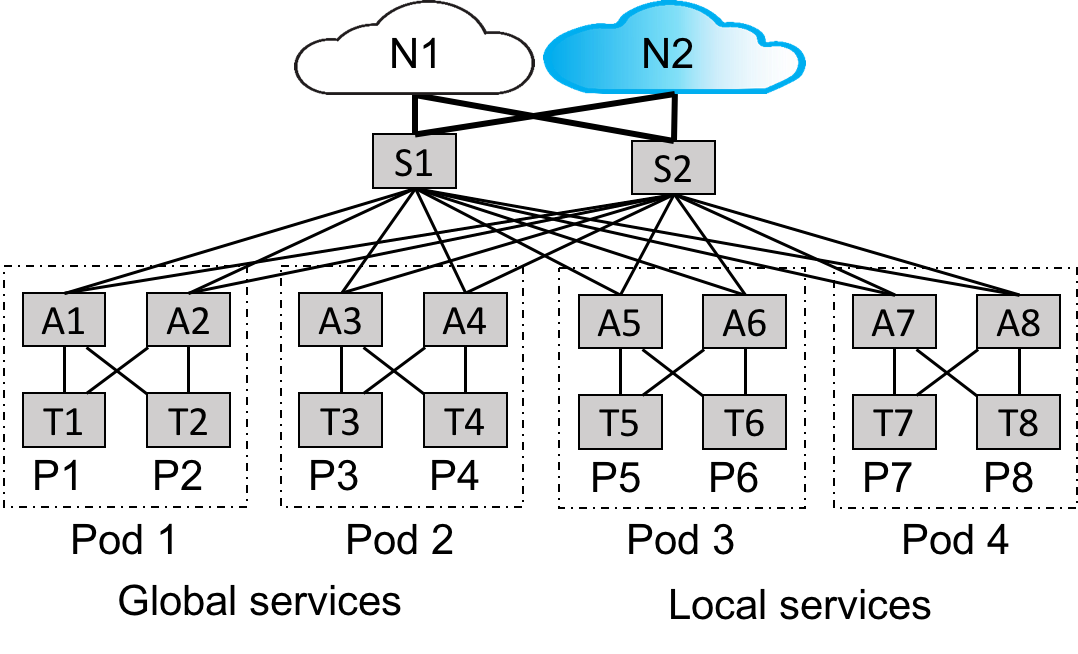
\includegraphics[width=2.5in]{figures/example}
  \vspace{-.8em}
  \caption{An example data center network.}
  \label{fig:example}
  \vspace{-.8em}
\end{figure}

The intended policy for this network is:
$(1)$ complete internal connectivity, \IE, all routers should be able to reach each other;
$(2)$ services in Pods[1--2] should be accessible from outside;
$(3)$ prefixes for global service should be aggregated into a covering prefix PG when announced outside;
$(4)$ services in Pods[3--4] should not be externally accessible;
$(5)$ traffic paths should be valley-free (\EG, a path through S1 should
not go down through Ai and then back up through S2, for instance, 
creating an up-down-up path);
$(6)$ prefer neighbor N1 over N2, \IE, when both neighbors announce a prefix, send traffic through N1;
$(7)$ routers should not transit traffic between N1 and N2; and
$(8)$ no loss in connectivity after any single-link failure.

\begin{figure}[t!]
  \centering
  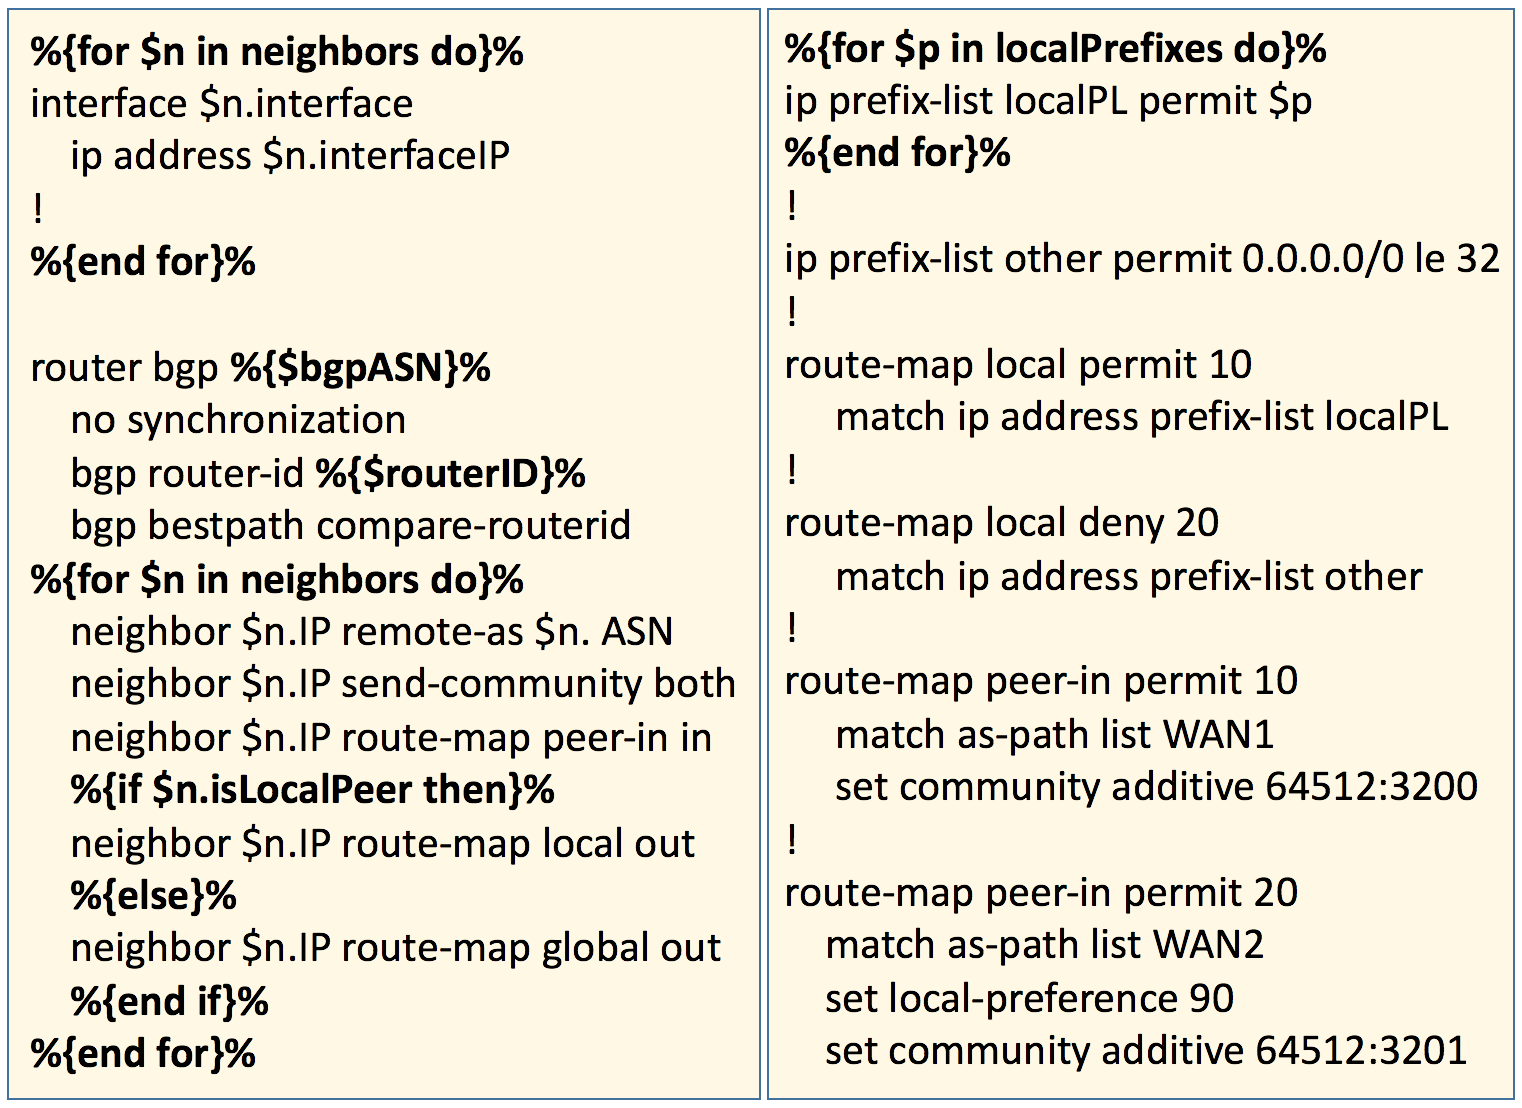
\includegraphics[width=\columnwidth]{figures/templates}
  \caption{Idealized small configuration component for the data center spine based on templates from a cloud provider.}
  \label{fig:templates}
  \vspace{-.8em}
\end{figure}


To correctly configure this policy, operators must generate configurations for each router, which implies ensuring, for instance, that all routing adjacencies are correctly configured (\EG, T1's configuration includes A1 as neighbor and vice-versa); the ToRs announce the correct prefixes for their services; all routers  forward the prefix announcements that they should to each neighbor and not forward others (\EG, the spines should forward prefixes for local services to internal neighbors but not to external neighbors); and the spines announce externally only the covering global prefix. Such configuration tasks are highly complex~\cite{juniper-study,bgpmon,batfish,propane}.

To simplify them, operators are adopting a template-based approach~\cite{hatch,thwack}. Instead of authoring a configuration per router, operators author a template per role.
%
A {\em role} is a specific function that is served by one or more routers.
%\footnote{If a role is played by devices from multiple vendors, there is one template per role-vendor combination because templates use vendor configuration languages.}
%
For example, the network in Figure~\ref{fig:example} might have five roles: spine, global aggregator, global ToR, local aggregator, and local ToR.
%
Figure~\ref{fig:templates} shows an example of what a small component of a template for the spine role in the two data centers might look like. The template has parameters for various aspects of the configuration (\EG, neighbor list, local prefixes) and is compiled to low-level device configurations by instantiating the parameters using the network topology and a database of network information.

%Templates provide two key advantages. First, they help eliminate a class of configuration errors that stem from typos and inconsistencies, e.g., using the wrong address for a router, having inconsistent addresses for the two ends of a link, and failing to configure one side of a routing adjacency.  Second, templates have the potential for re-use when the topology changes while maintaining its basic structure (e.g., adding a new pod to the data center) or multiple networks with similar structures need to be instantiated (e.g., in an organization that runs multiple data centers).

As described earlier (\S\ref{sec:introduction}), templates are hard to author and hard to validate. Worse, templates that work for one topology may not work for seemingly-inconsequential variations which may arise after the network evolves.
Consider the network in Figure~\ref{fig:example2}, which is similar to Figure~\ref{fig:example}; it has the same five roles, connected in a similar hierarchy. One might think that the same templates, with different database entries, can be used for both cases. However, if the templates are configured to disallow ``valley" paths (per policy (5) above), they will work for Figure~\ref{fig:example} but silently violate the fault tolerance policy $(8)$ when used for Figure~\ref{fig:example2}.  Specifically, in Figure~\ref{fig:example2}, an aggregation-based black hole (\S\ref{sec:background}) will occur when the link S1--A1 fails; after this failure, S1 has no valley-free path to P[1--2] even though it will continue to get traffic for these prefixes as it announces the covering prefix PG (because it gets routes for P[3--4]). Such a black hole will not occur in Figure~\ref{fig:example} because spine routers have two links to each pod.

%Unfotunately, currently, there is no way to predict which variations will behave correctly for a given set of templates.

\begin{figure}[t!]
  \centering
  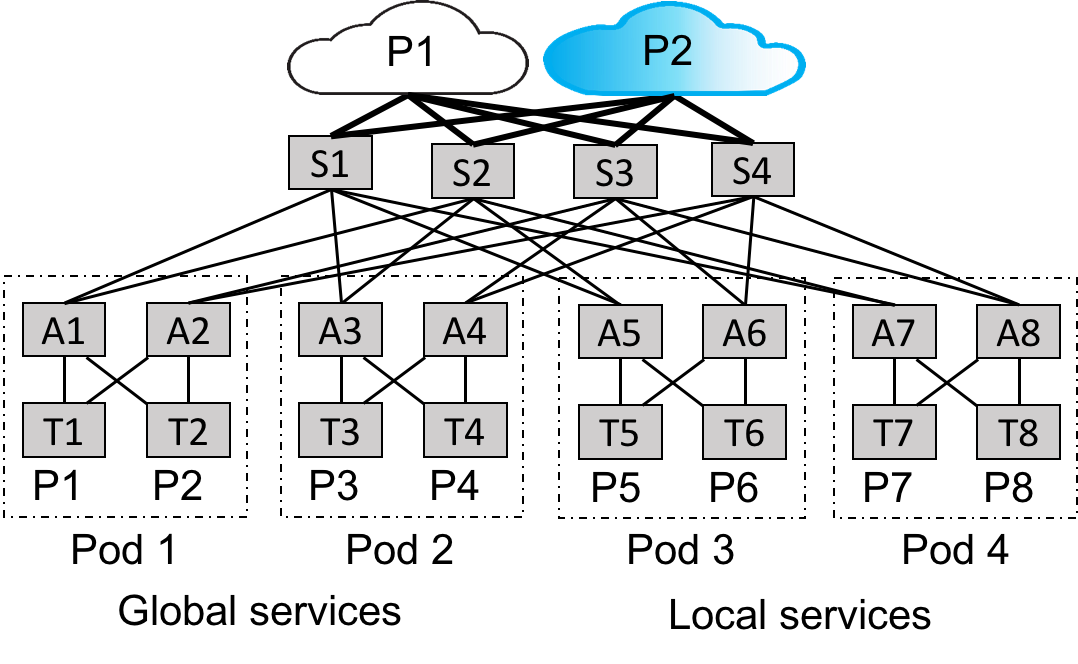
\includegraphics[width=2.5in]{figures/example2}
  \vspace{-.8em}
  \caption{A modified version of the network in Figure~\ref{fig:example}.}
  \label{fig:example2}
  \vspace{-.8em}
\end{figure}


When operators discover that an old template no longer works, they may consider changing it, which may cause a change to all devices that use it---an unacceptable disruption in many cases.  As a result, operators may abandon the template entirely and revert to hand-crafting configuration patches to accommodate the change.
Such patches reintroduce the complexity and the risk of errors that templates were meant to prevent.


%they are difficult to author. Operators must manually decompose complex, network-wide routing policy into role templates such that the collective behavior of the configurations generated from them will correctly implement the policy, both when failures occur and as the network evolves.

%This task is error-prone, and no tools exist today for template verification; in fact, such tools would be difficult to build as templates have no semantics, of policies or topologies they were intended to work for, independent of the configurations they produce. Today, operators test (not verify) templates by simulating their generated configurations over the current or known future topologies.

%As a result, the types of configuration design errors pointed in prior work~\cite{propane} can occur in template design as well. For instance, to keep local prefixes internal the engineer may implement announcement forwarding on spines based on the identity of the neighbor, \IE, do not announce externally anything heard from local aggregators. This implementation is appealing because it does not require changes to spine configurations when ToR prefixes change. But it works correctly only when there are no failures; local prefixes can leak externally when failures disconnect a spine from both aggregators in a local pod. Specifically, when S1 is disconnected from A5 and A6, it may hear about P5 and P6 from A3 and A4 (via A[5--6]->S2->A[3--4]), and it will then announce those prefixes outside (since they no not come from a local aggregator), leading to a policy violation. A possible correct implementation here would be for each spine to block messages headed to external peers from local aggregators {\em and} to reject announcements that have traversed the other spine (\IE, to disallow "valleys," or up-down-up paths).

%Lacking correctness guarantees, engineers use simulations to analyze if templates are correct under a range of failure cases (e.g., combinations of two-link failures), but such analysis is highly expensive for large networks and still does not provide strong guarantees beyond the tested cases.

%The second limitation of today's template systems is that, like concrete synthesis tools, they do not support network evolution. One might hope that important network properties such as connectivity and fault tolerance persist when networks evolve in ways consistent with existing roles and templates.  However, existing template systems provide no guarantees that seemingly-minor variations of a given topology have similar properties.
%In theory, templates do not have to be redesigned when the network evolves while keeping its basic structure of roles and their inter-connectivity. In practice, however, it is not guaranteed that templates that work for a given topology also work for seemingly-minor variations of the topology.

%Such simulations provide some assurance that the templates work correctly for the simulated topologies but little assurance for other topologies that may arise after the network evolves.

%Templates that work for one topology may not work for seemingly-inconsequential variations.
%Unfotunately, currently, there is no way to predict which variations will behave correctly for a given set of templates.
%Worse, when operators discover their old templates no longer work, changing a template will
%cause a change to all devices that use that template---an unacceptable disruption in many cases.  When that happens, operators may abandon templates entirely and revert to hand-crafting configurations, using local patches to accommodate the change.
%Such patches reintroduce the complexity and errors that templates were meant to prevent.

%% For some changes, they may discover that their old templates will not work anymore. ~\dpw{Note: This is going to be true for Methane too.} ~\ratul{Not really; our abstract topologies encode all possible future topologies} ~\dpw{Our abstract topologies precisely define a set of topologies for which our
%% This discovery is highly problematic because changing a template may cause a configuration change of all the devices that use that template---an unacceptable disruption in many cases.  When that happens, network operators may abandon templates entirely and revert to hand-crafting configurations, using local patches to accommodate the topological change.
%% Such patches reintroduce the complexity and errors that templates were meant to prevent.


%% Thus, today, operators test templates for each topology change. For some changes, they may discover that their old templates will not work anymore. ~\dpw{Note: This is going to be true for Methane too.} ~\ratul{Not really; our abstract topologies encode all possible future topologies} ~\dpw{Our abstract topologies precisely define a set of topologies for which our
%% This discovery is highly problematic because changing a template may cause a configuration change of all the devices that use that template---an unacceptable disruption in many cases.  When that happens, network operators may abandon templates entirely and revert to hand-crafting configurations, using local patches to accommodate the topological change.
%% Such patches reintroduce the complexity and errors that templates were meant to prevent.


%\para{Configuration synthesis with concrete topologies}
%Many recent systems generate router configurations using high-level policy statements~\cite{narain:lisa05,narain+:configassure,dadc,propane} and the network's concrete topology.
%%These systems eliminate entire classes of configuration errors by construction, and, in the case of
%%\Propane~\cite{propane}, guarantee that high-level policy is implemented correctly, even in the presence of
%%arbitrary combinations of failures.
%They are able to provide strong guarantees on configuration correctness but
%our conversations with operators at two major cloud providers reveal that they have two limitations that discourage adoption.  The first is abstraction mismatch. Operators of large networks think of the network, and develop management tools, using \emph{roles}, and not individual devices. They are naturally reluctant to use a system that does not
%understand roles as a first-order abstraction. If they want to debug, analyze or
%understand system output, they will have to consider
%\emph{hundreds} of independent device configurations instead of just
%\emph{a handful} of role configurations. Unfortunately, even if two devices play the same role,
%there is no guarantee a concrete synthesis system will generate (syntactically) similar configurations.
%
%%A second limitation is the inability to support network evolution. Networks evolve all the time as nodes and links are added or removed and the addresses of services are changed. A system that supports evolution would ensure that
%%small changes in topology require small, local changes in network configurations as opposed to pervasive
%%changes across many devices.  Engineers want to minimize changes to device configurations because each change runs the risk of poor, transient behavior due to poor router software or routing protocol dynamics~\cite{ratulbgpmisconfigs}.
%%These networks must be highly
%%available; it isn't plausible to bring down an entire data center network, or large portions of it, to make
%%incremental changes.
%
%Second, these systems become even more brittle in the face of network evolution.
%Any change in network topology requires re-execution of a
%concrete synthesis engine, from scratch,
%on the changed topology.  The result may be
%a completely different set of configurations.  Even if such configurations are
%largely semantically similar to existing configurations, they may be syntactically different and cause considerable network disruption when updates are pushed to routers.

%For instance, suppose an operator wants to modify the prefix of local ToR T8 in Figure~\ref{fig:example}. To accommodate the modification, \Propane, a concrete synthesis tool, will, at a minimum, not only change T8's configuration but also those of the two spines because it uses prefix lists at spines to ensure that local prefixes are not advertised externally.  As we show later, there is a way to design the configurations of this network to avoid spine configuration changes while accommodating ToR prefix (and other) modifications.  Our new abstraction-based synthesis framework synthesizes evolution-friendly roles automatically.

%nof the new spine configurations outputted by \Propane will not only enable the interfaces that connect to the new aggregators but will also have to update the prefix list filters. A system that supports incremental growth should need only interface configuration changes (not filter changes). It can configure all local ToRs, including the new ones, to attach a tag to their announcements and filter external announcements at the spines based on this tag. Engineers prefer fewer configuration changes because each change runs the risks of poor transient behavior (which synthesis tools do not reason about).


%For instance, suppose the engineers want to add another pod with local services to the network in Figure~\ref{fig:example}. In this network, \Propane, a concrete synthesis tool, uses prefix lists at spines to ensure that local prefixes are not advertised externally. To accommodate the expansion, the new spine configurations outputted by \Propane will not only enable the interfaces that connect to the new aggregators but will also have to update the prefix list filters. A system that supports incremental growth should need only interface configuration changes (not filter changes). It can configure all local ToRs, including the new ones, to attach a tag to their announcements and filter external announcements at the spines based on this tag. Engineers prefer fewer configuration changes because each change runs the risks of poor transient behavior (which synthesis tools do not reason about).

%As an aside, a possible template implementation that works correctly for both networks is: allow valley paths and use an explicit list of local prefixes at spines to decide which announcements should not be forwarded externally.

%\begin{figure}
%\begin{tabular}{|p{0.6in}|p{0.6in}p{0.7in}p{0.6in}|}
%\hline
%& Abstract Roles & Correctness Guarantees & Evolution Support  \\ \hline
%Concrete Synthesis & \xmark & \cmark & \xmark \\ \hline
%Template Systems & \cmark & \xmark & \xmark \\ \hline
%\sysname & \cmark & \cmark & \cmark \\  \hline
%\end{tabular}
%\caption{Comparing configuration techniques.}
%\label{fig:marketing}
%\end{figure}

%\subsection{\sysnamesec}
%
%As Table~\ref{fig:marketing} shows, \sysname addresses the limitations of both concrete synthesis and current template systems. It operates at the right level of abstraction for network operators, provides strong guarantees about compiled configurations, supports verification of important correctness properties, and supports network evolution.

%=====================================================
%
%
%  **Methane Overview**
%
%
%=====================================================

\section{Propane/AT overview}
\label{sec:overview}

%In this section we give an overview of \sysname, a system for generating provably-correct templates from the network's policy and an {\em abstract} topology that describes device roles and connectivity invariants.
%As inputs, it takes a global, network-wide policy (as opposed to a per-device or even per-role policy) and an {\em abstract} topology that describes device roles and connectivity invariants.  It outputs a template for each role, from which per-device configurations can be generated by instantiating parameters with values drawn from the network topology.
%It guarantees that:
%(1) the configurations generated from its templates correctly implement the network's policy for {\em any} concrete topology that matches the abstract topology; and (2) if nodes or edges are added or removed in a way compatible
%with the abstract topology, only configurations of devices adjacent to the change ever need to be updated.
%
%This section introduces \sysname using the examples in \S\ref{sec:motivation}.
%, and the following sections detail template generation and formally define the correctness guarantees.
%
%When \sysname generates templates, it guarantees that the forwarding behavior of the network will be correct for any instantiation of the templates on a concrete network that repects the abstraction.
%Furthermore, \sysname will generate configurations in such a way that, if an operator expands their network in a way compatible with the abstraction, then only configurations of devices adjacent to the change ever need to be updated.


%\subsection{Inputs}

\sysname takes as input the network's abstract topology and its policy. The policy consists of the routing policy that describes how traffic should flow and the fault-tolerance policy that describes how many simultaneous link failures the network should withstand without losing connectivity.

\para{Abstract topology}
Abstract topologies in \sysname define structural and role-based invariants that compactly describe all concrete networks that can emerge as the network evolves. They are encoded in the form of a graph homomorphism annotated with logical constraints about node and edge multiplicities.
%
We designed the abstractions to be able to precisely capture real network topologies, while being amenable to fault-tolerance analysis in the abstract domain.

%Ideally, we would like to find a suitable topology abstraction that can describe both of the data centers from figures~\ref{fig:example} and~\ref{fig:example2} as well as any reasonable generalization of these data centers. \sysname provides several abstraction mechanisms to achieve this goal.

%We introduce our topology abstractions using the networks from \S\ref{sec:motivation}.
Our topology abstractions consist of several concepts.
The primary one is a role-based abstraction that allows an operator to map routers in the concrete network to roles in the abstract network. Figure~\ref{fig:example3} shows an example of this abstraction for both networks from \S\ref{sec:motivation}. In the example, the concrete networks are abstracted into a new topology with 5 different roles: local ToR (TL), global ToR (TG), local aggregator (AL), global aggregator (AG), and spine (S).

\begin{figure}[t!]
  \centering
  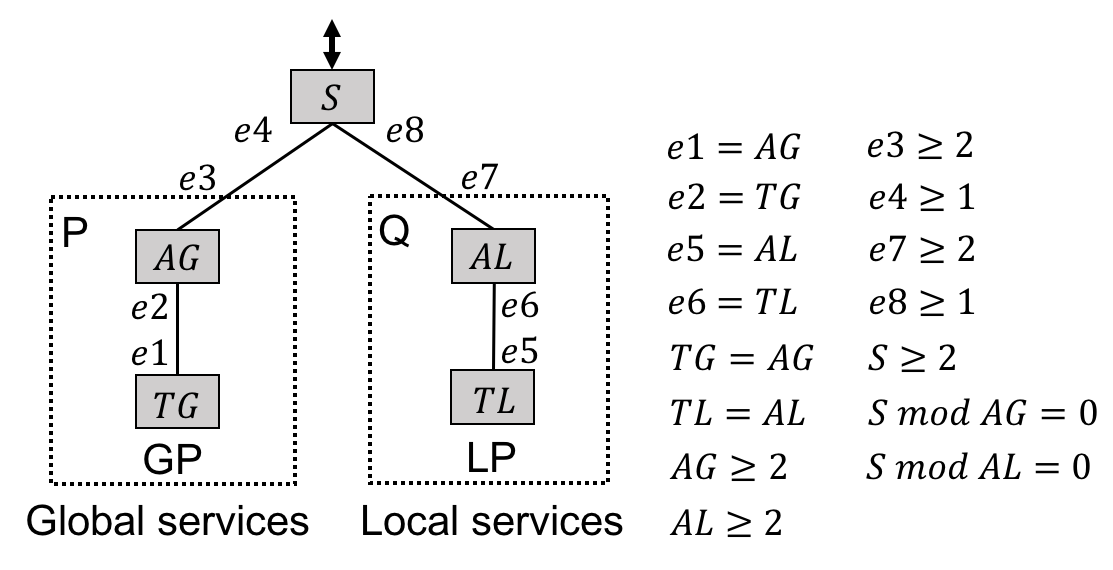
\includegraphics[width=\columnwidth]{figures/example3}
  \vspace{-1.3em}
  \caption{An abstraction for the network in Figure~\ref{fig:example}.}
  \label{fig:example3}
  \vspace{-.6em}
\end{figure}

More specifically, a network topology is a graph $G$ = ($V, E$), which consists of a set of vertices $V$ and a set of directed edges $E \colon V \times V$. A role-based abstraction is a graph homomorphism from $G$ to an abstract graph $G^A$ = ($V^A$,$E^A$). A graph homomorphism $f : G \rightarrow G^A$ maps each node in the concrete graph to a node in the abstract graph such that, whenever $(u,v) \in E$, then $(f(u),f(v)) \in E^A$. The role-based abstraction therefore over-approximates the connectivity of the underlying concrete graphs.

On its own, this abstraction loses a lot of information about the concrete network's structure, making it difficult to reason precisely about fault-tolerance.
%which would hinder a useful analysis of its fault-tolerance.
For example, with this abstraction any spine router may or may not connect to any aggregator router.
%
To capture concrete networks more precisely,
we introduce additional concepts. The first is topology hierarchy, captured by P and Q, which indicate that nodes in the ToR and aggregator roles are grouped into pods.
The second is node and edge \emph{multiplicity}. Each edge (and node) is labelled
with a symbolic variable (\EG, $e1$) that denotes a constraint on the number of edges (and nodes) that may appear in any valid concrete network. Operators can capture concrete network invariants by adding constraints on the symbolic variables using logical formulas.

For example, in Figure~\ref{fig:example3}, the first constraint ($e1 = AG$) 
%and
states that, within any pod P, the number of outgoing edges from a node in the 
$TG$ role (\IE, $e1$) to a node in the $AG$ role equals the number of nodes in the 
$AG$ role. Similarly, the constraint ($e2 = TG$) states that the number of 
outgoing edges from a node in the $AG$ role (\IE, $e2$) to a node in the $TG$ role 
equals the number of nodes in the $TG$ role. Together these constraints capture 
the fact that, within any pod, the global aggregators and ToRs are in 
a full mesh. Furthermore, the constraints $AG = AL$ and $AG \leq S$ ensure 
that, within pods P and Q, the $AG$ and $AL$ roles have the same number of 
routers, which is less than or equal to the number of routers in the spine 
role $S$.
%
The constraint $e3 \geq 2$ says that, in each pod, each aggregator node has at least 2 outgoing edges to nodes in the spine role. Symmetrically, the constraint $e4 \geq 1$ says that, for each pod P, each node in the spine role has at least one outgoing edge to a node in the $AG$ role. Similar constraints appear for the local aggregator role. The constraint $2 \leq S \leq 4$ makes explicit the possibility for growth, for example, by growing the network from Figure~\ref{fig:example} to Figure~\ref{fig:example2}. In general, we need not bound the number of spine routers to admit more concrete topologies, potentially at the expense of analysis precision. We also include the constraints $(S \mod AG) = 0$, and $(S \mod AL) = 0$~simply to show that constraints do not have to be in the form of inequalities. Operators can use logical formulas from any theory supported by modern SMT solvers.

A final concept is the $\Mincut(1)$ constraint between the spine role S and N[1--2]. It says that any spine router has at least one path to any node in the neighbor N1 (and N2) role. Such annotations are useful for a ``one big switch" abstraction \cite{Casado:2010} in which a complex, unstructured network is represented as a single node. As another use case, an ISP backbone can be modeled by dividing the network into separate geographic regions with two roles per region---one for the border routers and another for the network core. Mincut annotations can describe the degree of fault tolerance both within regional cores and across regions.

Our topology abstractions can also capture concrete topologies by using a one-to-one correspondence between abstract and concrete nodes/edges. This allows operators to define complex networks in which some (e.g., legacy) parts of the network cannot evolve while others can.
%It also means that our compiler subsumes those that operate only over concrete topologies.

%All the guarantees provided by \sysname hold for any instantiation of the abstract network. This means that operators can safely expand their network in the future so long as the new network also satisfies these logical constraints.

%Although the concrete \sysname policy can help prevent a number of configuration errors,
%the policy is intricately linked to the actual structure of the concrete network.
%For example, each prefix in the routing constraint is enumerated with its concrete destination
%location, and the definition of the valleyfree constraint depends on the actual routers that
%comprise each tier of the data center.
%
%This is unfortunate since any expansion of our data center network will require a corresponding
%change to the policy. Furthermore, there is no guarantee that a safe policy can be found
%for the expanded network, and even if one can be found, it may require changes to every
%configuration in the network -- a huge barrier to adoption in practice.

%Abstract \sysname solves this problem in two ways. First, it allows operators to abstract
%the network into a role-based topology and write a routing specification over this abstraction instead.
%Second, it introduces prefix template variables into the language to allow writing policies that are
%parameterized over prefix destination.

\para{Routing policy} Routing policies in \sysname consist of an ordered sequence of $i)$ a predicate that matches a class of traffic; and $ii)$ paths that the traffic should take through the network, ranked per their relative preference. \sysname borrows syntax from \Propane~\cite{propane}, but instead of concrete predicates and paths, uses abstract predicates and paths.

Let us see how to express the routing policy of the networks in \S\ref{sec:motivation} over the abstract topology. We can capture the basic routing behavior, constraints (1, 2, 6),  as follows:
%
\begin{code}
\Define Routing =
    \$GP  \Path \End(TG)
    \$LP  \Path \End(TL)
    \True \Path \End(\Out) & \Exit(N1 \Prefer N2)
\end{code}
\noindent%

The second line introduces a prefix \emph{template} variable $\CD{\$GP}$. Template variables represent multiple instances of a rule for different concrete prefixes that can be provided by an external source (\EG, a database). The line says that traffic for each global prefix associated with the variable should follow a path that ends at its corresponding destination router in the $\CD{TG}$ role. As we will see in \S\ref{sec:language}, constraints like $\CD{\End(TG)}$ are just syntactic sugar for regular expressions describing network paths. The second line has a similar policy for local prefixes.
%
The final rule matches all other IP prefix destinations and allows traffic to follow a path that leaves the data center, ending at some external role ($\CD{\Out}$), through neighbors $\CD{N1}$ or $\CD{N2}$ with a preference for leaving through $\CD{N1}$. The $\CD{\Prefer}$~symbol indicates that traffic should satisfy the constraint on the left and resort to the backup (right) only when that is not possible due to network failures.%

Next, we can capture constraint (4) that traffic for local prefixes must stay within in the data center:
%
\begin{code}
\Define Local =
    \$LP \Path \Always(\In)
\end{code}
\noindent%
%
The \CD{Local} policy adds the $\CD{\Always(\In)}$ constraint for each local prefix described by the template variable $\CD{\$LP}$. This constraint ensures that traffic follows a path that matches an internal role (\IE, in the data center) at each hop of the path.
%
The constraint to prevent ``valleys" (5) is written as:
%
\begin{code}
\Define NoValley =
    \True \Path \Novalley(\{TG,TL\},\{AG,AL\},\{S\})
\end{code}
\noindent%
%
This policy applies to all traffic and prevents valley paths by adding the $\Novalley$ constraint with arguments corresponding to each level in the data center.
%
Constraint (7) to prevent transit traffic between neighbors is expressed as:
%
\begin{code}
\Define Peer = \{N1,N2\}
\Define NoTransit =
    \True \Path !(\Enter(Peer) & \Exit(Peer))
\end{code}
\noindent%
%
We define a $\CD{Peer}$ as $\CD{N1}$ or $\CD{N2}$ and disallow paths where traffic both enters and exits the data center through a peer.

Finally, we can combine these constraints together as:

\begin{code}
Routing & Local & NoTransit &
NoValley & \Agg(GP_AGG, \In -> \Out)
\end{code}
\noindent
This instructs \sysname to satisfy the conjunction of all the constraints. It also declares that we want to perform route aggregation, with covering prefix {\small GP\_AGG}, for global prefixes at the border of the data center (\IE, along any edge that connects the inside of the data center to the outside). In this case, {\small GP\_AGG} is declared as a concrete prefix rather than a template because a single aggregate prefix will be used to summarize all less-specific prefixes.

\para{Fault-tolerance policy} This policy specifies how many link failures the network should be able to withstand before traffic experiences connectivity loss. Operators can specify different tolerance levels for different pairs of abstract nodes. For instance, they may say that ToR to spine connectivity should be robust to 2 failures, \IE, no ToR-spine pair should lose connectivity as long as the number of simultaneous link failures is 2 or fewer; and ToR-to-ToR connectivity should be robust to 1 failure.

% The \text{} is needed for some reason for formatting
\para{Synthesis} \sysname generates templates from the inputs above in three phases. First, it combines the abstract topology and routing policy into a {\em product graph} (PG) that compactly captures the flow of routing information over the topology in a policy-compliant manner. The algorithm for this phase builds on \Propane (for concrete networks); we show that it can be extended to abstract inputs.
%and that the extensions are correct.

Second, \sysname checks if the fault-tolerance policy can be met by considering the joint impact of the abstract topology and routing policy. Joint analysis is needed, because connectivity depends on both: traffic will not flow along valid topological paths if the routing policy disallows it.
%
We develop a sound analysis based on computing the minimum
number of edge-disjoint, policy-compliant paths between pairs of nodes
over abstract topologies. If this number is less
than the desired fault-tolerance level for a pair of nodes, \sysname declares that the
policy cannot be met.
%\ryan{Possibly cut here}
%More specifically,
%for each abstract role in the network, our analysis will learn facts about the
%number of disjoint paths to routers in that role.  For example,
%the fact $A_{S}(2,3)$ states that for \emph{all} groups of 2 nodes
%in the $S$ (Spine) role, there are 6 disjoint paths to the group---3
%for each of the 2 nodes. A fact such as $S_{S}(2,3)$, states that
%\emph{some} group of 2 nodes has the property as opposed to all.
%More generally, there is one quantifier ($A$ for all groups
%and $S$ for exists a group).  When nodes are nested within pods,
%there is one quantifier for each level of the hierarchy, so
%$S_P S_{TG} (i,j)$ means that for some pod from the $P$ group of pods
%and for some nodes in the $TG$ role within that pod, there exists a
%group of $i$ nodes with $j$ paths to each node in the group.

%\ryan{Possibly cut here}
%As an example, suppose we want to compute the number of of disjoint paths between any global ToR and spine router in Figure~\ref{fig:example3}.
%The analysis begins with the fact
%$S_P S_{TG} (1,1)$---there is some group of
%nodes of size 1 in the $TG$ role in some pod $P$ such that any initial
%node in the $TG$ role has 1 disjoint path to it (and all such paths are
%edge-disjoint). Since the abstract topology specifies that each node in
%the $TG$ role is in
%a full mesh with nodes in the $AG$ role within any given pod, we
%infer the fact $S_P A_{AG}(e1,1)$. This says that
%any group of nodes of size e1 in the $AG$ role is reachable with at
%least 1 path to each such node from any initial node in
%the $TG$ role.
%
%After one more step, the analysis will learn a fact of the form $A_{S}(1,1)$, which means that any single spine node is reachable via a single disjoint path from any initial global ToR node
%In fact, due the valley-free routing constraint, a single path is
%the worst-case fault-tolerance level for the concrete network from
%Figure~\ref{fig:example2}.

If it can be met, \sysname generates templates for each node in the abstract topology.  Per-device BGP configurations can in turn be generated from the templates
using information in the concrete topology. To ensure the process is sound,
\sysname checks that the given concrete topology is an instance of the abstract topology.

The following sections detail each of the three phases.

%
%The constraint prevents traffic from over taking a path that traverses
%either [Agg->Tor->Agg] or [Spn->Agg->Spn]. The final policy remains the same as before,
%by combining each of these policies together.
%
%


%=====================================================
%
%
%  **Language and Product Graph**
%
%
%=====================================================

\section{Product Graph Generation}
\label{sec:language}


\begin{figure}[t]\small
  \begin{minipage}[t]{\linewidth}
  \vspace*{-1\baselineskip}
  %
  \[ \begin{array}{rclr}
     d       &\in& \textit{Integers} \\
     x       &\in& \textit{Variables} \\
     l       &\in& \textit{Topology Locations} \\
     pol     &::=& p_1, \dots, p_n & \text{Policy} \\
     p       &::=& t \hspace{.3em} \Path \hspace{.3em} r_1 \Prefer \dots \Prefer r_m \BNFALT a & \text{Path Preferences}  \\
     t       &::=& \$x \BNFALT d.d.d.d/[d..d] \hspace{1.5em} & \text{Predicate} \\
     a      &::=& \mathit{agg}(t, r_1 \rightarrow r_2) & \text{Aggregation} \\
     r       &::=& l \BNFALT \emptyset \BNFALT \CD{in} \BNFALT \CD{out} \BNFALT r_1 \cup r_2 \BNFALT & \text{Regular Path} \\
             &   & r_1 \cap r_2 \BNFALT r_1 \cdot r_2 \BNFALT \NOT r \BNFALT r^* \\
  \end{array} \]%

  \end{minipage}
  \vspace{-.4em}
  \caption{\sysname core syntax.}
  \label{fig:syntax}
  \vspace{-0.8em}
\end{figure}%




\newcommand{\state}[4]{\node[state,#3](#1)[#4]{#2};}
\newcommand{\transition}[4]{\path[->] (#1) edge [#4] node {#3} (#2);}

\begin{figure*}[t!]
  \begin{minipage}[t]{.4\linewidth}
  \hdr{Policy Automata}{}
  \vspace{1em}
    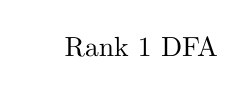
\begin{tikzpicture}[>=stealth',shorten >=1pt,auto,node distance=2cm,minimum size=.5cm]
      \state{0}{$0$}{              }{}
      \state{1}{$1$}{right of=0}{accepting}
      \transition{0}{0}{out}{loop above}
      \transition{0}{1}{N1}{}
      \transition{1}{1}{in}{loop above}
      \node at (1,-1){Rank 1 DFA};
    \end{tikzpicture}
    ~~~~~
    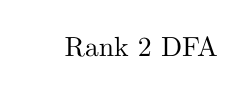
\begin{tikzpicture}[>=stealth',shorten >=1pt,auto,node distance=2cm,minimum size=.5cm]
      \state{0}{$0$}{              }{}
      \state{1}{$1$}{right of=0}{accepting}
      \transition{0}{0}{out}{loop above}
      \transition{0}{1}{N2}{}
      \transition{1}{1}{in}{loop above}
      \node at (1,-1){Rank 2 DFA};
    \end{tikzpicture}%
  \end{minipage}
  %
  ~~~~~~
  %
  \begin{minipage}[t]{.3\linewidth}
    \hdr{Concrete Topology}{}
    \vspace{1em}
    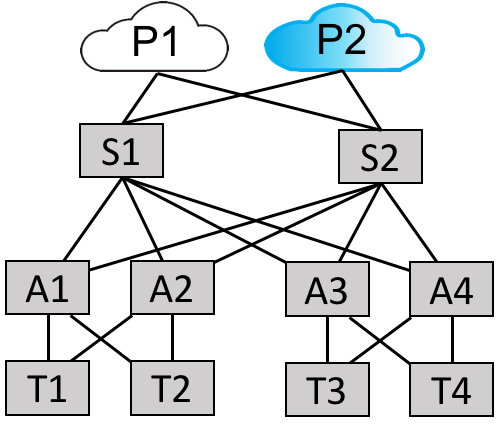
\includegraphics[width=.60\columnwidth]{figures/topology-con}
  \end{minipage}%
  %
  \begin{minipage}[t]{.3\linewidth}
    \hdr{Abstract Topology}{}
    \vspace{1em}
    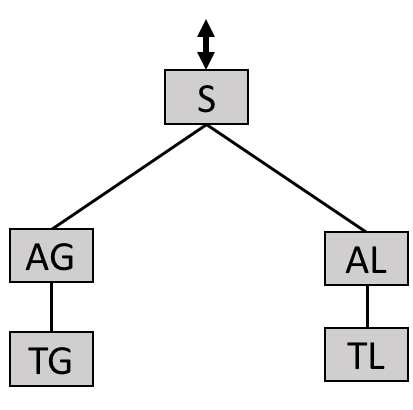
\includegraphics[width=.49\columnwidth]{figures/topology-abs}
  \end{minipage}%

  \vspace{1em}
  \begin{minipage}[t]{.6\linewidth}
    \hdr{Concrete Product Graph}{}
    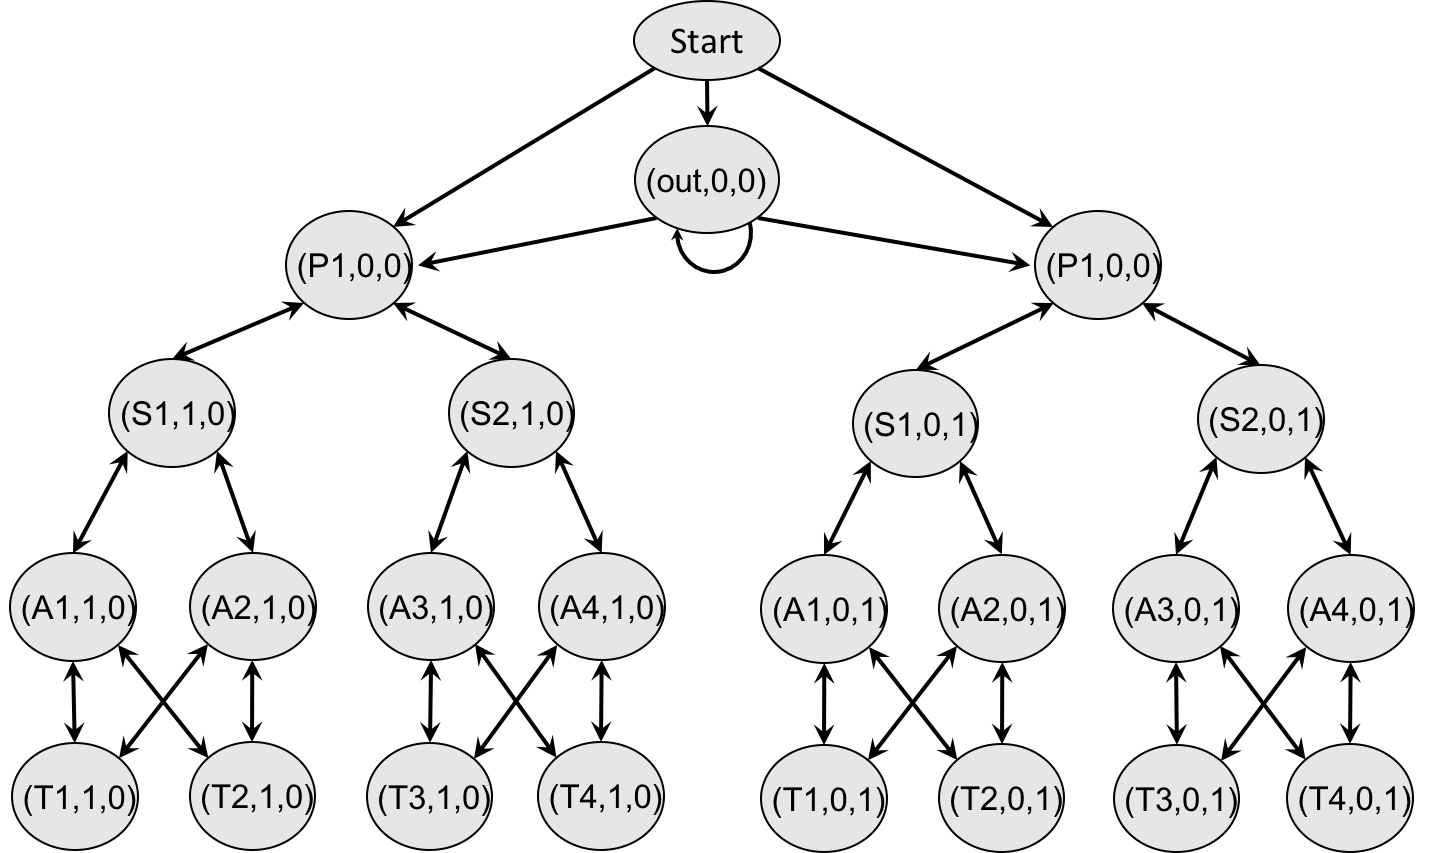
\includegraphics[width=.8\columnwidth]{figures/pg-con}
  \end{minipage}%
  \begin{minipage}[t]{.4\linewidth}
  \hdr{Abstract Product Graph}{}
    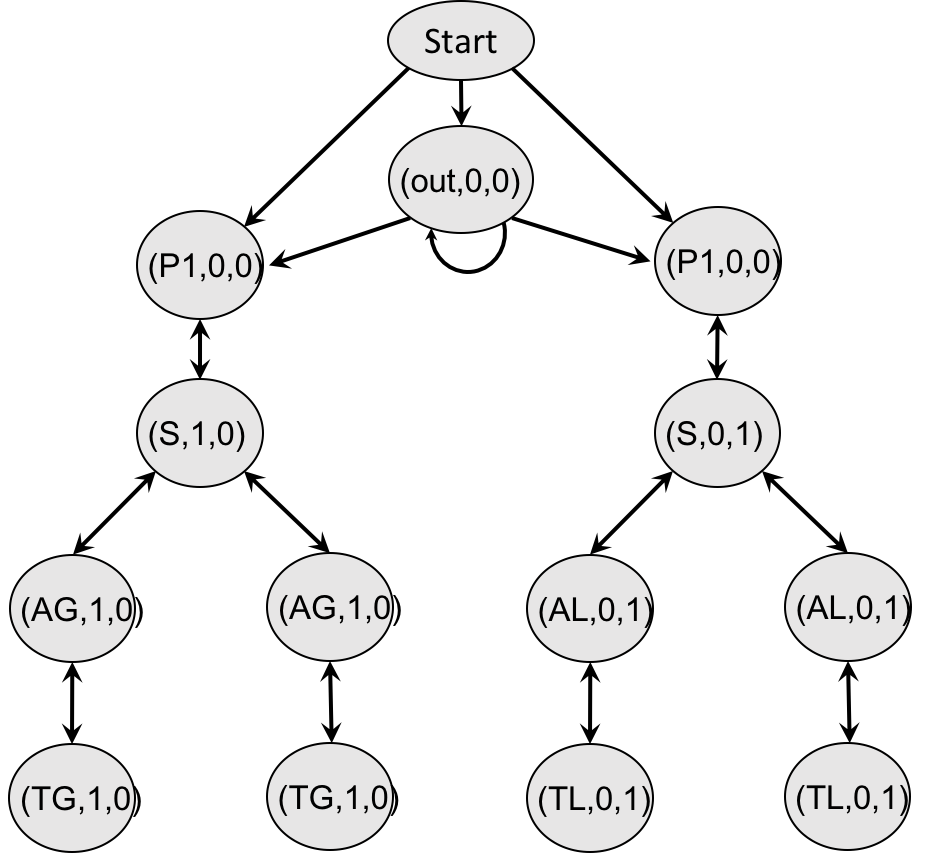
\includegraphics[width=.795\columnwidth]{figures/pg-abs}

  \end{minipage}%

  \hrulefill
  \vspace*{-.4em}%
  \caption{Product Graph construction for policy $\True ~\Path~ \CD{\Exit(\text{N1}} ~\Prefer~ \CD{\text{N2})}$.}
  \label{fig:example-compilation}
  \vspace{-.8em}
\end{figure*}


The first step for the \sysname compiler is to build the product graph (PG), a data structure that is amenable to joint analysis of the topology and routing policy. As a precursor to this step, we convert the routing policy syntax in \S\ref{sec:overview} to a core language based on regular expressions, shown in Figure~\ref{fig:syntax}.
%
A policy has one or more constraints, each an aggregation or a path constraint. Path constraints have a test on a destination prefix and a list of regular expressions describing network paths. Regular paths are defined over network locations, where each location is either a router inside the operator's network, or an external neighbor connected to that network. Values \In\ and \Out\ will match any internal and external location respectively. There are two types of predicates, as shown. A test for a concrete prefix $d.d.d.d/[d..d]$ matches a range of IP prefixes (\EG, 10.0.1.0/[24..32]) where metavariable $d$ represents an integer. A prefix template test {\small\$x}, for variable $x$, represents a collection of many tests, one for each prefix represented by the template.

Converting from the high-level syntax from \S\ref{sec:overview} to the core syntax is straightforward. The predicate $\True$ becomes the prefix range $0.0.0.0/[0..32]$.
%
Each constraint desugars to a regular expression. For example, the constraint $\Always\CD{(\In)}$ becomes $\In^*$ and the constraint $\CD{\End(TG)}$ becomes $\mathtt{\Sigma}^* \cdot \CD{TG}$.
%
Preferences are lifted to the top level of the regular expression when their use is unambiguous, and separate sets of constraints are joined prefix-by-prefix by taking the regular expression intersection of their constraints.

%For example, the combining the Routing and Local constraints in the data center policy from \S\ref{sec:overview} would result in the following \sysname policy:
%
%\begin{code}
%\$PG  \Path \End(TG),
%\$PL  \Path \End(TL) \ensuremath{\cap} \Always(\In),
%\True \Path \Exit(Peer1) \Prefer \Exit(Peer2)
%\end{code}
%\noindent%
%

%After converting the routing policy to the regular expression based language,
We are now ready to generate the PG. Intuitively, the PG captures topology and routing constraints by ``intersecting" the finite automata associated with the policy regular expressions with the graph structure of the topology.
%The PG compactly encodes all paths that protocol messages should be passed along through the network in order to guarantee that the BGP-speaking devices find policy-compliant paths dynamically.
%
%Although \sysname policies describe the routes that traffic should take through the network, network protocols (including BGP) typically disseminate router information in the opposite direction. For example, a router Y will tell its neighbor X that it has a route to the destination meaning that X can send traffic through Y. For this reason, we start by compiling
%
Because there can be a separate routing policy for each predicate $t$ in the policy, we construct one PG for each predicate.


For each regular path constraint $r_i$ from $r_1 ~\Prefer~ ... ~\Prefer~ r_k$, we construct a DFA for the reverse of $r_i$. A DFA for $r_i$ is defined as a tuple ($\Sigma, Q_i, F_i, q_{0_i}, \sigma_i$). The alphabet $\Sigma$ is the set of topology locations (\IE, routers or roles), $Q_i$ is the set of states for automaton i, $F_i$ is the set of final states, $q_{0_i}$ is the initial state, and $\sigma_i \colon Q_i \times \Sigma \rightarrow Q_i$ is the state transition function.
%
The PG for a graph (\IE, a topology) $G=(V,E)$ is a tuple ($G'$, $start$, \Pref) where $G' = (V',E')$ has
vertices $V' \colon V \times Q_1 \times \dots \times Q_j$,
edges $E' \colon V' \times V'$,
a unique starting vertex $start$,
and a ranking function $\Pref \colon V' \rightarrow 2^{\set{1, \dots, j}}$, mapping nodes in the PG to a set of path ranks.

The PG is constructed by adding an edge from state $m = (l_m, q_{m_1}, \dots, q_{m_k})$ to $n = (l_n, q_{n_1}, \dots, q_{n_k})$ whenever $\sigma_i(q_{m_i}, l_n) = q_{n_i}$ for each $i$ and $(l_m,l_n) \in E$.
%
We add edges from the $\mathit{start}$ node to any $m = (l, q_{m_1}, \dots, q_{m_k})$ when $\sigma_i(q_{0_i}, l) = q_{m_i}$ for each $i$.
%
The ranking function $\Pref(m)$ denotes the rank of paths through the PG ending at node $m$ and is defined as $\Pref(m) = \set{i~\vert~q_{m_i} \in F_i}$.
%
Finally, we write $\Topo{m} = l$ to extract the topology location from a PG node, when $m = (l, q_{m_1}, \dots, q_{m_k}) \in V'$. For the remainder of the paper, we use the term \emph{location} to refer to a router in the case of a concrete topology/PG, or a role in the case of an abstract topology/PG.

Figure~\ref{fig:example-compilation} shows the PG for the data center policy that applies to all external traffic ($\CD{\True \Path \Exit(N1~\Prefer~N2)}$).
%
%\begin{code}
%\True \Path \Exit(\sf{Peer1}) \Prefer \Exit(\sf{Peer2})
%\end{code}
%\noindent%
%
The first automaton represents the more preferred constraint $\CD{\Exit(N1)}$ and the second automaton represents the less preferred constraint $\CD{\Exit(N2)}$. The PG is shown for both an instance of a simple concrete network matching the abstraction from \S\ref{sec:overview} as well as for the abstract topology.

Paths through the PG represent paths through the topology that BGP announcements may use to ensure policy-compliance. For example, in the concrete PG, all messages from N1 are not blocked at spine routers S1 and S2. Paths for a destination learned through N1 will end in an accepting state for the first automaton (\EG, node (T1,1,0)). Similarly, paths for a destination learned through N2 will end in an accepting state for the second automaton.

Interestingly, the concrete and abstract PGs have a similar structure, which leads to the following observation:

\begin{lem}
\label{lem:homomorphism}
If we have a graph homomorphism $f : G \rightarrow G^A$, concrete product graph $PG = (G',\mathit{start},\Pref)$ and abstract product graph $PG^A = (G'^A, \mathit{start}^A, \Pref^A)$, then there is a homomorphism $f_{pg} : G' \rightarrow G'^A$ where:
\[ \begin{array}{rcl}
  f_{pg}( \mathit{start} ) & = & \mathit{start}^A  \\
  f_{pg}( (l,q_1,\ldots,q_n) ) & = & (f(l),q_1,\ldots,q_n) \\
\end{array} \]
\end{lem}
%
As shown in \S\ref{sec:generation}, our generation strategy commutes with template instantiation, meaning that we obtain the same results if we instantiate the abstraction early, or if we defer the instantiation until after template generation.
%
%Lemma~\ref{lem:homomorphism} provides intuition as to why our strategy for generating templates is correct.
%Abstract product graphs are related to concrete product graphs via a graph homomorphism, just as abstract topologies are related to concrete topologies via a graph homomorphism.



%=====================================================
%
%
%  **Abstractions**
%
%
%=====================================================


\section{Fault-tolerance Analysis}
\label{sec:analysis}

%In practice, operators would often like to reason about a variety of properties for, not only their current network topology, but also future versions of it.
%% The Product Graph provides a convenient representation to capture the joint impact of both topology and routing policy. In this section we present an analysis that operates over the abstract Product Graph to find a lower bound on the number of disjoint paths between pairs of concrete nodes. Answering questions about the number of disjoint paths between nodes allows operators to reason about many useful network properties such as reachability (\IE, is there at least one path) and fault tolerance (\EG, how many failures will disconnect certain routers).


%\subsection{Abstract k-disjoint paths}
%\label{sec:property-checking}

The possibility of network failures exacerbates the difficulty of constructing correct configurations.
Link failures in networks occur frequently; it is not uncommon for a large network to experience dozens of failures in any given day~\cite{dc-failure-study}. However, existing tools~\cite{condor,propane} reason about fault-tolerance only for concrete topologies. \sysname provides stronger guarantees: all possible concrete instantiations of an abstract topology satisfy the fault-tolerance policy.

%The problem for \sysname is harder because it must verify that all possible concrete instantiations of an abstract topology satisfy the fault-tolerance policy, which requires a fundamentally different approach.

%
We frame satisfying the fault-tolerance requirements as an analysis problem over the structure of the PG. In particular, we develop an analysis that uses information embedded in the abstract topology to infer bounds on the number of edge-disjoint paths between pairs of concrete nodes.

%
For each node in the abstract PG,
the idea is to infer facts learned about the number of edge-disjoint paths
to groups of concrete routers in the node's role.
More specifically, we maintain fact of the form:
%
\[ \begin{array}{c}
  L_{X_1}, \ldots, L_{X_n}(j,k)
\end{array} \]
\noindent
%
where each label $L \in \{S,A\}$ is either $S$, which stands for ``some" or is $A$, which stands for ``all". There is one label for each pod in the abstraction pod hierarchy under which the abstract node appears. For a given node, $L_{X_1}$ corresponds to the outermost pod, $L_{X_{n-1}}$ corresponds to the innermost pod, and $L_{X_n}$ to the node itself.
Semantically, $L_{X_1}, \ldots, L_{X_n}(j,k)$ means that starting from some concrete source node, for some/all pods $X_1, \ldots, X_{n-1}$
and for some/all groups of nodes in the role $X_n$ of size $j$,
%, $L_{X_2}, \ldots, L_{X_n}(j,k)$ holds. The base case $L_{X_n}(j,k)$ means that for "some"/``all" groups of size $j$ concrete routers,
there are $k$ paths to each such that all $j*k$ paths are edge-disjoint.

For example,
an inference of the form $A_{Q} A_{TL}(2,3)$ states that, from the given source location, for \emph{all} pods Q, and \emph{all} groups of 2 nodes in the TL role, there are 6 disjoint paths to the group---3 for each of the 2 nodes.



\newcommand{\inference}[7]{
    \node[draw, anchor=west] at (#1 + .5, 2.5 / 2) {#3};
    \node[] at (#1, 2.5 / 2 + 2.5) {\textbf{#5}};
    \node at (#1 + .34, .6 + .2) {#6};
    \node at (#1 + .34, 1.9 - .2) {#7};
    \node at (#1, -.6) {#2};
    \node at (#1, 2.5 + .4 + .2) {#4};
    \draw [] (#1, 2.5 - .2) circle [radius=0.4] node {$n$};
    \draw [] (#1, .2) circle [radius=0.4] node {$m$};
    \draw [->] (#1, .4 + .2) -- (#1, 2.5 - .4 - .2);
}

\newcommand{\inferencenobox}[7]{
    \node[anchor=west] at (#1 + .1, 1.25) {#3};
    \node[] at (#1, 2.5 / 2 + 2.5) {\textbf{#5}};
    \node at (#1 + .34, .6) {#6};
    \node at (#1 + .34, 1.9) {#7};
    \node at (#1, -.6) {#2};
    \node at (#1, 2.5 + .4 + .2) {#4};
    \draw [] (#1, 2.5 - .2) circle [radius=0.4] node {$n$};
    \draw [] (#1, .2) circle [radius=0.4] node {$m$};
    \draw [->] (#1, .2 + .4) -- (#1, 2.5 - .4 - .2);
}

\newcommand{\derivation}[3]{
    \node at (#1, -.6) {#2};
    \node at (#1, 3.1) {#3};
    \node at (#1, -.6 + .9) {$\mathcal{E}$};
    \node at (#1, 3.1 - .9) {$\mathcal{D}$};
    \node at (#1, 2.5/2) {.};
    \node at (#1, 2.5/2 - .26) {.};
    \node at (#1, 2.5/2 + .26) {.};
}

\newcommand{\inferencetwo}[1]{
    \node[draw, anchor=west] at (#1 + 2, 1.25) {$e_i > 0$};
    \node[] at (#1 + .46, 1.25 + 2.5) {\textbf{I-striping}};
    \node at (#1 - 1 - .11, .6 + .2) {$e_1$};
    \node at (#1 + .11, 1.5 + .2) {$e_2$};
    \node at (#1 + 2 + .11, .6 + .2) {$e_3$};
    \node at (#1 + .11 + .8, 1.5 + .2) {$e_4$};
    \node at (#1 - 1, -.8 + .2) {L$_m(j,k)$};
    \node at (#1 +. 5, 2.9 + .2) {S$_n(min(j*k,g),1)$};
    \node at (#1 + 2, -.8 + .2) {S$_o\big( min(j, g *\frac{e_4}{e_3}),1\big)$};
    \node at (#1, 3.3 + .2) {};
    \draw [] (#1 + .5, 2.01 + .2) circle [radius=0.4] node {$n$};
    \draw [] (#1 - 1, 0 + .2) circle [radius=0.4] node {$m$};
    \draw [] (#1 + 2, 0 + .2) circle [radius=0.4] node {$o$};
    \draw [->] (#1 - 1, .4 + .2) -- (#1 + .5, 2 - .4 + .2);
    \draw [<-] (#1 + 2, .4 + .2) -- (#1 + .5, 2 - .4 + .2);
}

\newcommand{\inferencelocal}[2]{

    \node[] at (#1 + 1.2, 1.25 + 2.5) {\textbf{I-local}};
    \derivation{#1}{X}{Y}
    \derivation{#1+2+#2}{L$_P$ X}{L$_P$ Y}
    \node[anchor=east] at (#1 + .5 + #2, 2.5 / 2) {$\Rightarrow$};
    %\inferencenobox{#1}{X}{}{Y}{}{}{}
    %\inferencenobox{#1+2 + #2}{$\ldots$ L$_P$ X}{}{$\ldots$ L$_P$ Y}{}{}{}
    \node[anchor=east] at (#1 + 2 + #2 - .6, 2.5) {P};
    \draw[dashed] (#1+1 + #2 - .2, -.34) rectangle (#1+3 + #2 + .1, 2.85);
}

\newcommand{\inferenceglobal}[2]{
    \node[] at (#1 + 1.2, 2.5 / 2 + 2.5) {\textbf{I-global}};
    %\inferencenobox{#1}{X}{}{Y}{}{}{}
    %\inferencenobox{#1+2+#2}{L$_P$ X}{}{A$_Q$ Y}{}{}{}
    \derivation{#1}{X}{Y}
    \derivation{#1+2+#2}{L$_P$ X}{A$_Q$ Y}
    \node[anchor=east] at (#1 + .5 + #2, 2.5 / 2) {$\Rightarrow$};

    \node[anchor=east] at (#1 + 2 + #2 - .6, .4) {P};
    \node[anchor=east] at (#1 + 2 + #2 - .6, 2.5) {Q};
    \draw[dashed] (#1+1+#2 - .2, -.34) rectangle (#1+3+#2 + .1, .8);
    \draw[dashed] (#1+1+#2 - .2, 1.7) rectangle (#1+3+#2 + .1, 2.85);
}

\begin{figure*}[t!]
  \begin{minipage}[t]{\linewidth}%
  \begin{tikzpicture}
    \inference{0}{L$_m(j,k)$}{$e_1 > 0$}{S$_n(min(j*k,e_1),1)$}{I-out1}{$e_1$}{$e_2$}
    \inference{3.5}{A$_m(j,k)$}{$e_2 > 0$}{A$_n(1,min(j,e2))$}{I-out2}{$e_1$}{$e_2$}
    \inference{7}{L$_m(j,k)$}{$e_1=n$}{A$_n(min(j*k,n),1)$}{I-mesh1}{$e_1$}{$e_2$}
    \inference{10.5}{L$_m(j,k)$}{$e_1=n$}{A$_n(1,j)$}{I-mesh2}{$e_1$}{$e_2$}
    \inferencenobox{14}{L$(j,k)$}{$\Mincut(X)$}{A$(1,min(k,X))$}{I-mincut}{}{}
  \end{tikzpicture}
  \end{minipage}

  \vspace*{.2em}
  \begin{minipage}[t]{\linewidth}%
  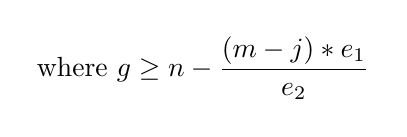
\begin{tikzpicture}
    % \inference{0}{L$(j,k)$}{$e_i > 0$}{S$(min(j*k,g),1)$}{I-out3}{$e_1$}{$e_2$}
    \inferencetwo{0}
    \node[anchor=west] at (1,2.2) {where $g \geq n-\dfrac{(m-j)*e_1}{e_2}$};
    \inferencelocal{6.5}{.4}
    \inferenceglobal{12}{.4}
  \end{tikzpicture}
  \end{minipage}

  \hrule
  \vspace*{.4em}
  \caption{Abstract k-disjoint path analysis inference rules.}
  \label{fig:inference-rules}
  \vspace{-.8em}
\end{figure*}


\subsection{Inference rules}

\newcommand{\infrule}[1]{{\small \sf #1}\xspace}

Figure~\ref{fig:inference-rules} displays the collection of rules used to infer facts about disjoint paths.
Each rule is read from bottom to top. The label on the bottom left is a known fact. We use $L$ to represent a rule that is parametric over the label ($S$ or $A$). Labels on other nodes correspond to facts learned after applying the rule. The box shows the conditions that must be valid, given the abstraction constraints, for the rule to apply. 
%Validity ensures that the condition holds for all concrete instantiations of the topology.

Some of the inference rules (\EG, \infrule{I-out2} and \infrule{I-mesh2}) try to learn about the largest number of disjoint paths to any single node in an abstract role, while others (\EG, \infrule{I-out1} and \infrule{I-mesh1}) try to learn about the largest reachable group in a particular role with at least one disjoint path to each node in that group. Both kinds of rules are useful. 

The first rule, \infrule{I-out1} applies to a learned fact of the form $L_m(j,k)$ where the number of outgoing edges from any concrete node in the $m$ role is greater than 0. In the worst case, the largest group of concrete nodes we could hope to reach at the $n$ role would be $e_1$ since all j nodes at the bottom may have outgoing edges to the same concrete nodes at the top. Furthermore, the total number of disjoint paths to the $j$ nodes at the bottom is equal to $j*k$. Since extending the existing disjoint paths with disjoint edges keeps the paths disjoint, and since we cannot exceed the current number of disjoint paths to the concrete nodes in role $m$ on the bottom, the largest reachable group for the role $n$ on the top will be $min(j*k,e_1)$.
%
We conservatively use $1$ for the number of disjoint paths to each node in role $n$, since when $n$ is very large, all reachable nodes in role $m$ might only have a single edge to completely different nodes in $n$.
%However, because we do not know for certain that all $j$ nodes in role $m$ have outgoing edges to the same nodes at the top, we conservatively use $1$ for the number of disjoint paths to each node on top.
%For example, if $n$ is very large, then each node in role $m$ may have only a single edge to each reachable node in role $n$.

Consider rule \infrule{I-out2}, and consider any node in the role $n$. There are $e_2$ incoming edges to that node. Due to the fact that $A_m(j,k)$, we know that at least j of those $e_2$ edges are connected to nodes with disjoint paths from the origin. Hence we infer $A_n(1,min(j,e_2))$.

%The rule \infrule{I-out2} follows a similar line of reasoning. It says that if any group of size $j$ with $k$ disjoint paths to each is reachable in the bottom role, and there is at least one incoming edge for each concrete node in the top role, then there are $min(j,e_2)$ disjoint paths to any single concrete node in the top role. This is because we can choose the $j$ nodes on the bottom for which we want to find disjoint paths, and then use each of the $e_2$ disjoint incoming edges for the particular node at the top connecting it to the bottom.

The two rules \infrule{I-mesh1} and \infrule{I-mesh2} handle the case where there is a full mesh between the two roles. This happens when the number of outgoing edges ($e_1$) from nodes in role $m$ equals the number of nodes on top ($n$). \infrule{I-mesh1} says that we can find disjoint paths to each node in the top role restricted to the number of disjoint paths we started with. \infrule{I-mesh2} uses the fact that each node in the top role is connected to each node in the bottom role to infer that there can be $j$ disjoint paths to any single node in the top role.

The annotation $\Mincut(X)$ appearing on an edge is an assertion about the fault tolerance between nodes in two different roles. The rule \infrule{I-mincut} uses such assertions. To each node in role $n$, from a node in role $m$, we can construct at least the minimum of $X$ and $k$ disjoint paths.

%The rule \infrule{I-mincut} can be thought of as an assertion about the fault tolerance between nodes in two roles. The rule applies to an edge that has been annotated with a $mincut(X)$ statement, which means that there are at least $X$ disjoint paths between any node in role $m$ and any node in role $n$.

The rule \infrule{I-striping} is the most complicated case.
It starts with the invariant $L_m(j,k)$ at role $m$ and can be applied if each edge multiplicity $e_i > 0$ is valid given the constraints. The first inference for role $n$ tries to find the largest reachable group with disjoint paths to each. The idea is similar to the rule \infrule{I-out1}, but is able to use the fact that $e_2 > 0$ to learn more about the structure of the concrete topology. In particular it uses the following inequality, where $g$ represents the size of the group for the role $n$:
%
\[ \begin{array}{c}
  (m-j)*e_1 \geq (n-g)*e_2
\end{array} \]
\noindent
%
The remaining nodes ($m-j$) that are not part of the reachable group in the bottom role, each have $e_1$ outgoing edges and must be able to at least ``fill" the incoming edges for the remaining nodes not in the reachable group at the top ($n-g$), which each have $e_2$ incoming edges. Solving the inequality gives the lower bound for $g$ used in Figure~\ref{fig:inference-rules}.

The second part of the rule uses a similar idea to reason about the overlap between roles $m$ and $o$ with respect to role $n$. This rule is particularly useful for data center topologies where routers in one tier of the data center often have a uniform striping pattern with another tier.

Finally, rules \infrule{I-local} and \infrule{I-global} reason across pod hierarchies. \infrule{I-local} says that if there is an inference from $X$ to $Y$, then the derivation can be used inside pod P by leaving the P-label unchanged. \infrule{I-global} says that when the edge goes across pods, we can infer the fact for all pods Q since the multiplicities apply uniformly for each pod.


\subsection{Inference algorithm}


The abstract disjoint path analysis starts from a fixed source location $src$ and repeatedly tries to apply every inference rule from Figure~\ref{fig:inference-rules} until it reaches a fixed point. The algorithm applies an inference rule when the rule's condition is valid given the abstract topology constraints. Because the inference rules may continue to yield larger and larger symbolic expressions, we make the following observation to ensure termination: for any invariant learned of the form $L(j,k)$, it is sound to instead infer $L(j',k')$ if $j' \leq j$ and $k' \leq k$. Therefore, for each inference $L(j,k)$ we minimize the symbolic expressions for $j$ and $k$ subject to the topology constraints using the optimizing SMT solver $\nu$Z~\cite{z3opt}. 

At a higher level, what is happening is that each inference rule is attempting to learn the maximum fault tolerance information possible as a function of the symbolic inputs. The $\nu$Z~\cite{z3opt} solver will then minimize this maximum by accounting for all possible topologies that meet the abstraction. Facts learned with $j=0$ or $k=0$ are discarded.

%The algorithm associates with each inference, the set of abstract locations used to derive the inference, \IE, an overapproximation of set of concrete locations used for the edge-disjoint paths. When applying an inference rule between an invariant at role $m$, with a set of abstract locations $C$, to learn an invariant at role $n$, we associate the new invariant with the set $C \cup \{ n \}$.
%
%When, at a single PG node there is an inference $L_{X_1} \dots L_{X_{n-1}}$ A$_m(j,k)$ with location set $C$ and inference $L_{X_1} \dots L_{X_{n-1}}$ L$_m(j',k')$ with location set $D$, where $C \cap D = \emptyset$, we add a new inference with location set $C \cup D$:
%
%$$L_{X_1} \dots L_{X_{n-1}} L_m(\min(j, j'), k + k')$$
%
%\noindent
%The idea is that, because non-overlapping abstract paths can never contain overlapping concrete paths, due to the graph homomorphism property, we can merge inferences about these disjoint paths in the abstraction.

\begin{figure}
  \begin{center}
    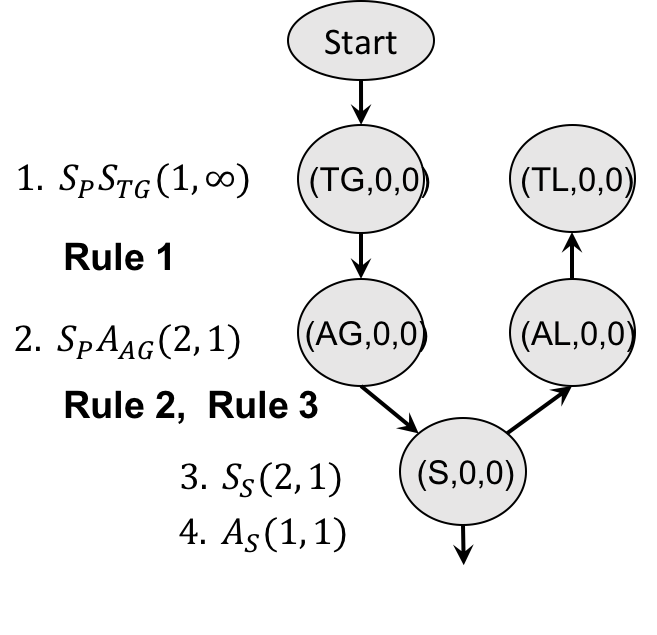
\includegraphics[width=\columnwidth]{figures/analysis}
  \end{center}
  \vspace{-1em}
  \caption{Abstract disjoint path analysis for global prefixes. \label{fig:compilation-times}}
  \label{fig:example-inference}
  \vspace{-.8em}
\end{figure}

Recall the policy for global prefixes in the data center.
%
\begin{code}
\$GP \Path \End(TG) \ensuremath{\cap}
       \Novalley(\{TG,TL\},\{AG,AL\},\{S\}) \ensuremath{\cap}
       !(\Enter(Peer) & \Exit(Peer))
\end{code}
\noindent
%
Figure~\ref{fig:example-inference} shows part of the abstract PG representation for this routing policy. The inference algorithm starts from the node $(TG,0,0)$ with the initial fact $S_P S_{TG}(1,\infty)$ (\IE, no restriction on the number of disjoint paths initially).
%
The first step applies each inference rule to this initial fact. The algorithm uses rules \infrule{I-mesh1} and \infrule{I-local} to reason about connectivity within a single pod for the TG and AG roles. It makes a call to $\nu$Z to minimize the expression $min(\infty, AG)$, which results in 2. Therefore, the algorithm learns a new invariant of the form $S_P A_{AG} (2,1)$ for node $(AG, 0)$ to indicate that in some pod P, any group of 2 nodes is reachable.
%
The algorithm will then eventually apply \infrule{I-out2} to learn that any single spine node is reachable at $(S,0)$. It will also apply \infrule{I-striping} to determine that there is some group of at least 2 spine routers reachable at $(S,0)$ and that there is some group of at least 2 nodes reachable in the AL role in state $(AL,0)$.

Note that, because each inference rule only applies to directed edges in the PG, the algorithm cannot make any inferences about connectivity from the AL role to the S role since there is no directed edge from AL to S. This restriction ensures that the analysis remains policy-sensitive.

The next step is to use \infrule{I-mesh2} together with \infrule{I-local} to infer that any single node in the TL role for any pod Q is reachable via at least 2 disjoint paths. This process will continue until a fixed point is reached.

The algorithm could infer that there is at least 1 disjoint path to any spine router, and at least 2 disjoint paths to any TL router. In this case, the analysis is precise. There exists a concrete network, namely the data center from Figure~\ref{fig:example2}, where a single failure can disconnect a global ToR from a spine router due to the valley-free constraint.
%The bound on the fault tolerance between ToR and spine routers can also be used to determine that an aggregation-induced black hole may arise at the data center boundary after a single failure in some concrete instantiation.


%=====================================================
%
%
%  **Compilation to BGP**
%
%
%=====================================================

\newcommand{\highlight}[1]{%
  \colorbox{red!50}{$\displaystyle#1$}}
\newcommand{\Router}[1]{\KW{Router} #1:}
\newcommand{\Template}[1]{\KW{Template} #1:}
\newcommand{\REGEX}[1]{\texttt{regex}(#1)}
\newcommand{\PEER}{\texttt{peer}}
\newcommand{\PREFIX}{\texttt{prefix}}
\newcommand{\IF}{\texttt{if}}
\newcommand{\THEN}{\texttt{then}}
\newcommand{\COMM}{\texttt{comm}}
\newcommand{\MED}{\texttt{MED}}
\newcommand{\Arrow}{\ensuremath{\leftarrow}}



\section{Template Generation}
\label{sec:generation}

At a high level, the translation from the PG representation to per-device templates that run the distributed BGP protocol involves the following steps: (1) Every BGP message is tagged to record the state of the product graph as messages are passed between routers. The tags allow BGP to only search for valid paths by dropping messages that do not correspond to any edge in the PG. (2) To ensure that BGP always finds the \emph{best} paths in the network, we must rank route advertisements for each router locally such that, under this ranking function, the network as a whole satisfies the \sysname policy's end-to-end network preferences. 

We introduce a simple, vendor-independent BGP configuration language called \mbgp and describe a compilation function that uses the inferred preference ordering to generate concrete configurations from a concrete topology, or templates from an abstract topology. Given a concrete network, templates can be instantiated by replacing instances of abstract neighbors with the union of all concrete neighbors under the inverse homomorphism, and by replacing prefix template variables with separate entries for each concrete prefix provided by a context. 
 We call this process of transforming templates into configurations \emph{concretization}.  We prove that concretization and compilation commute. Moreover, by modifying compilation slightly we can further ensure that every configuration depends only on its immediate neighbors. This guarantees that any change made to the concrete topology will result in a minimal number of changes to the configurations.
%
We now look at each of these steps in turn.
 

\para{Tagging and Filtering}

The BGP routing protocol allows \emph{community tags}---32-bit integer tags that can be arbitrarily attached to, or removed from, routing advertisements. 
Community tags serve as a simple form of \emph{history}, and operators routinely use such tags to implement policy. For example, operators might tag advertisements at certain entry points and then block the export of tagged 
advertisements to prevent their network from becoming a transit point.

Template generation uses community tags to record the state of the automata from the Product Graph in every BGP announcement and updates these tags whenever messages are passed between routers. This mechanism ensures that BGP only considers paths that are allowed by the \sysname policy (\IE, paths in the PG). Routers will allow advertisements that correspond to an edge in the PG and will block any advertisements that do not.

For example, in the concrete PG in Figure~\ref{fig:example-compilation}, router S1 appears in two PG nodes: $(S1,1,0)$ and $(S1,0,1)$. These nodes have two peers that can send them messages: $(N1,0,0)$ and $(N2,0,0)$. Therefore, S1 will allow advertisements from both peer $N1$ and peer $N2$. If S1 uses the path advertised by neighbor N1, then it will add the tag $(1,0)$ to the advertisement before sending this to its neighbors A1 and A2. If S1 uses a path advertised from neighbor N2, then it will add the tag $(0,1)$ instead. Similarly, router A1 appears in two PG nodes. It will admit advertisements that have the $(1,0)$ or $(0,1)$ tag attached (and drop all other advertisements). In either case, it will not modify the tag before exporting the route to its neighbors.

%\begin{algorithm}[t!]
%\caption{Checking safe neighbor preferences}
%\label{alg:failures}
%\begin{algorithmic}[1]
%\Procedure{$\leq$($N_1$, $N_2$)}{}
%  \If {$N_1 \not\approx N_2$} \Return false
%  \EndIf
%  \State $q \gets Queue()$
%  \State $q.Enqueue (N_1, N_2)$
%  \While {$!q.Empty()$}
%    \State $(m,n) \gets q.Dequeue()$
%    \If {$m \nleq_{rank} n$}
%      \Return false
%    \EndIf
%    \For {$n'$ in adjOut($PG$, $n$)}
%      \If {\big($\exists m' \in \textup{adjOut}(PG,m), m' \approx n'$\big)}
%        \If {$(m',n')$ not marked}
%          \State {mark $(m',n')$ as seen}
%          \State $q.Enqueue(m',n')$
%        \EndIf
%      \Else { \Return $false$}
%      \EndIf
%    \EndFor
%  \EndWhile \\
%  \hspace{\algorithmicindent} \Return true
%\EndProcedure
%\end{algorithmic}
%\end{algorithm}



\newcommand{\Con}{\text{con}}
\newcommand{\Pfx}{\mathit{pfx}}%

\vspace{2em}
\begin{figure*}[t!]\small%
  
  %\hrulefill%

  %\vspace{1em}%
  \begin{minipage}[t]{.47\linewidth}
  \hdr{mBGP Syntax}{}
  \vspace*{-1\baselineskip}
  %
  \[ \begin{array}{rclr}
     d    &\in& \textit{Integers} & \\
     c    &\in& \textit{Communities} & \\
     l    &\in& \textit{Topology Locations} & \\
     t    &::=& \$x \BNFALT d.d.d.d/[d..d] & \textit{predicate} \\
     ns   &::=& \{ l_1, ~\dots,~ l_k \} & \textit{peers} \\
     ma   &::=& d : ({ns}_1, c_1) \rightarrow ({ns}_2, c_2) & \textit{match action} \\
     pc   &::=& ma_1, \dots, ma_k & \textit{predicate config} \\
     rc   &::=& t_1 \rightarrow {pc}_1, ~\dots,~ t_k \rightarrow {pc}_k & \textit{router config} \\
     mbgp &::=& l_1 \rightarrow {rc}_1, ~\dots,~ l_k \rightarrow {rc}_k & \textit{mbgp policy} \\%
  \end{array} \]%%

  \end{minipage}
  %
  %
  \begin{minipage}[t]{.49\linewidth}
  \hdr{Compilation to mBGP}{}
  \vspace*{-1\baselineskip}
  %
  \[ \begin{array}{l}
     \mathrm{compile}_\mathrm{mBGP}( [(t_1,PG_1,pref_1), \dots, (t_k,PG_k,pref_k)], G ) = \\
     ~~~~~ [~ l \rightarrow rc ~\vert~ l \in \mathrm{internal}(G.V), ~rc = \mathrm{append}_i~  \\
     ~~~~~~~~~~~~~~~ [~ t_i \rightarrow [~ ma ~\vert~ \\
     ~~~~~~~~~~~~~~~~~~~~~ m \leftarrow (l,q_m) \in PG_i, \\
     ~~~~~~~~~~~~~~~~~~~~~ pin \leftarrow \mathrm{adjIn}(PG_i,m), \\
     ~~~~~~~~~~~~~~~~~~~~~ (in,q_n) \leftarrow \{ (bs,q_n) ~\vert~ bs=\{b ~\vert~ (b,q_n) \in pin \}, bs \neq \emptyset \}, \\
     ~~~~~~~~~~~~~~~~~~~~~ out \leftarrow \{ c ~\vert~ (c,\_) \in \mathrm{adjOut}(PG_i,m) \}, \\
     ~~~~~~~~~~~~~~~~~~~~~ ma = \mathrm{pref}_i(m) : (in,q_n) \rightarrow (out,q_m) ~] ~] ~] \\
     \\
     \mathrm{compile}( p_1, \dots, p_k, G) = \\
     ~~~~~~ \mathrm{compile}_\mathrm{mBGP}([\mathrm{compile}_\mathrm{PG}(p_1,G), \dots, \mathrm{compile}_\mathrm{PG}(p_k,G)], G) \\
  \end{array} \]%
  \end{minipage}%

  \vspace{1em}
  \hrulefill%
  \vspace{-.8em}
  \caption{mBGP syntax (left), and compilation from product graphs (right).}
  \label{fig:concretization}
  \vspace{-.4em}
\end{figure*}%


\para{Preference Search}

Tagging and filtering based on the PG restricts the possible paths to those that are allowed by the policy. However, finding \emph{some} path to the destination is not enough. We must ensure that each router uses its \emph{best} available path according to the policy. Further, each router must continue to use its best available path as elements of the network fail. In the example from Figure~\ref{fig:example-compilation}, the policy was $\True ~\Path~ \CD{\Exit(N1\Prefer N2)}$, which indicates that paths through N1 should be used whenever possible, and paths through N2 should only be used as a backup. If router S1 allows advertisements from both N1 and N2, but does not prefer one advertisement over another, it might end up choosing to use a path through N2 even though a more preferred path through N1 exists and is available\footnote{Ties between equally preferred paths can be broken nondeterministically.}. On the other hand, if the S1-N1 link fails, then the best available path is through N2.

To enforce correct path preferences, we use the BGP local-preference attribute, which allows routers to prefer certain routes (e.g., those from a particular neighbor or with a tag) over other routes. The challenge is to find a collection of device-local preferences that correctly enforce the policy's network-wide preferences in the face of any set of failures.

The idea is to search for such a device-local preference function for each router that totally orders advertisements from different neighbors (possibly with different tags). For example, to satisfy the policy that leaving through N1 is preferred to leaving through N2, S1 should prefer a message it hears from N1 over N2. Similarly, A1 should prefer routes tagged with $(1,0)$ over those with $(0,1)$. Intuitively, S1 should prefer a message from N1 because it results in an accepting state for automata 1, which indicates a better path. Further, it can result in downstream routers such as A1 using a path that is accepting for automata 1 as well.

In general, because BGP is distributed, each router does not have a view of the entire network when choosing which path to use, and finding a collection of preferences to ensure correct end-to-end behavior for all failures is a hard problem. \Propane introduced a conservative search strategy for determining route preferences that works well in practice. To make it work for abstract topologies, we modify the search based on the following observation about the PG structure:\footnote{Recall that $\Pref(m)$ is a set of priorities---those of the
automata whose final states include $m$.  
For instance, if $\Pref(m)$ is \{1,3\} then
automata 1 and 3 have $m$ as a final state.  Moreover, recall that
the policy expressed by automata $i$ is preferred to the policy expressed
by automata $j$ if $i < j$.}

\begin{defn}
Let $m \geq_{rank} n$ be a relation over PG vertices that holds iff $\Topo{m} = \Topo{n}$ and either $\min (\Pref(m)) \geq \min (\Pref(n))$ or $\Pref(n) = \emptyset$.
%
\end{defn}
\noindent
%
Intuitively $m \geq_{rank} n$ means that paths ending at node $n$ have lower automata rank and are thus better than paths ending at $m$.
%\begin{defn}
The PG can be viewed as a labelled transition system by pushing the location from each directed edge's target node onto the edge. That is, $m\overset{l}{\rightarrow}n$ if there is an edge $(m,n)$ in the PG and $\Topo{n} = l$.
%\end{defn}
%
For example, in the concrete PG we have the transition $(S1,1,0)\overset{A2}{\rightarrow}(A2,1,0)$.

\begin{defn}
We write $m \leq n$ if the subgraph reachable from $m$ and $n$ respectively form a simulation relation with respect to $\geq_{rank}$. More specifically, we say that $m \leq n$ if $n \geq_{rank} m$ and for every transition $n\overset{l}{\rightarrow}n'$ from PG node $n$ there exists a transition $m\overset{l}{\rightarrow}m'$ from $m$ and $m' \leq n'$.
\end{defn}


If $m \leq n$, then advertisements received for node $m$ can safely be preferred over those received for node $n$ after accounting for the network-wide impact of the choice. For example, in Figure~\ref{fig:example-compilation}, S1 can receive advertisements in two different contexts $(S1,1,0)$ and $(S1,0,1)$ and must choose between messages received in these different contexts. Advertisements are preferred in state $(S1,1,0)$ because they result in a better path for S1 ($(S1,0,1) \geq_{rank} (S1,1,0)$) and downstream routers such as A1 will also obtain paths no worse than if S1 had chosen $(S1,1,0)$. The policy is guaranteed to be safe from failures because if a link fails in the topology, then $m \leq n$ will still hold since any transition that becomes unusable for $m$ also becomes unusable for $n$. That is $m \leq n$ before the failure implies $m \leq n$ after the failure.

For each router, its corresponding PG nodes are then sorted according to the $\leq$ operator. If the operator defines a total order on PG nodes, then the compiler can simply prefer advertisements from peers of node $m$ over those of $n$ whenever $m \leq n$. However, if $\leq$ does not form a total order, then the policy is rejected as being potentially unsafe under some failure conditions.


%
For example, in Figure~\ref{fig:example-compilation} the inequality $(S1,0,1) \leq (S1,1,0)$ holds since nodes on the left side of the PG can always match transitions made on the right hand side with respect to the $\geq_{rank}$ relation. This relation does not hold the other way around since $(S1,0,1) \ngeq_{rank} (S1,1,0)$. Therefore, advertisements received at $S1$ with tag $(1,0)$ must be preferred to those received at $S1$ with tag $(0,1)$.
%
Notice that in the abstract PG $(S,0,1) \leq (S,1,0)$ also holds. This leads to the following observation:

\begin{lem}
\label{lem:preference}
$m \leq n$ in the concrete PG iff $f_{pg}(m) \leq f_{pg}(n)$ in the abstract PG.
\end{lem}

Lemma~\ref{lem:preference} tells us that inferring preferences for the abstract PG before template instantiation is equivalent to inferring preferences for an already-instantiated concrete PG.  A proof appears in the \Appendix.


\begin{figure}[t!]
  \begin{center}
    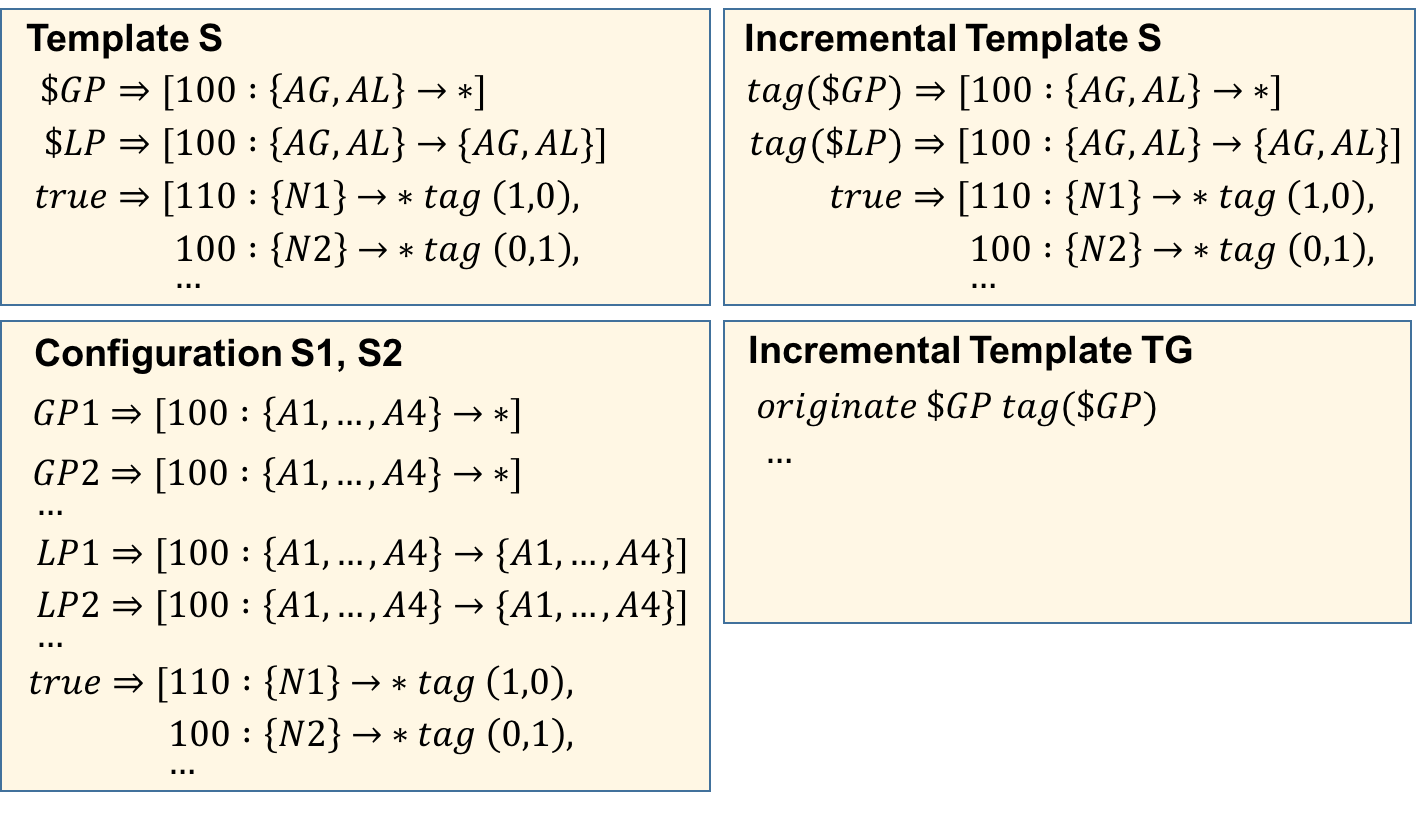
\includegraphics[width=\columnwidth]{figures/configs}
  \end{center}
  \vspace{-1em}
  \caption{Spine template and concrete configurations (left), and evolution-friendly templates (right).}
  \label{fig:bgp-configs}
  \vspace{-.6em}
\end{figure}

\para{mBGP}
To characterize compilation we first introduce a simple, vendor independent configuration language for the BGP protocol called \mbgp. The syntax for \mbgp is shown in Figure~\ref{fig:concretization} (left). An \mbgp policy consists of a sequence of router configurations (one for each internal topology location $l$). A router configuration is an ordered sequence of pairs, where is pair contains
a predicate describing the traffic, and a predicate configuration. A predicate is either a template variable $\$\mathrm{x}$ or a prefix. A predicate configuration is a collection of match action statements, where each match action indicates that the router will match advertisements from any of a set of peers $ns_1$ with a particular community tag $c_1$ with local preference $d$, before exporting the route to another set of peers $ns_2$ with a new community tag $c_2$.


\para{Compilation}

Figure~\ref{fig:concretization} (right) defines compilation from \sysname to \mbgp. It proceeds by compiling constraints $p_i$ in the original \sysname policy to a tuple of: the predicate $t_i$, the product graph $PG_i$, and the preference function $pref_i$. These tuples are passed to the $\mathrm{compile}_\mathrm{mBGP}$ function, along with the network topology $G$. For each internal router in the topology $l$, and each predicate $t_i$ in the \sysname policy, compilation goes through each node $m$ for $l$ in $PG_i$, and groups the inbound neighbors of $m$ by tag ($q_n$) into sets ($in$). It allows imports from these neighbors before exporting to the outbound neighbors of $m$. The local preference for these imports is given by $\mathrm{pref}_i(m)$, which represents an integer based on the total ordering of $(\leq)$. We build configurations using list-comprehension notation. For instance, $[~ l \rightarrow rc ~\vert~ l \in V, p(l,rc) ~]$ denotes the \mbgp policy $l_1 \rightarrow rc_{1},...,l_k \rightarrow rc_{k}$ where each $rc_{i}$ satisfies $p(l_i,rc_{i})$. We use $\mathrm{append}$ to denote sequence concatenation.%

Figure~\ref{fig:bgp-configs} (left) shows part of the generated \mbgp configuration for spine routers for both the concrete and abstract policies. For brevity, we using the symbol ($*$) to denote the set of all neighbors and omit tags when irrelevant.
%
For prefix $\True$, the spine routers will match advertisements from peer N1 and N2. The match for N1 is preferred since it has a higher BGP local-preference attribute (110). If an advertisement from N1 is chosen, the spine attaches the community tag $(1,0)$ before sending the route to all its peers ($*$). If an advertisement is only available from the backup N2, then it attaches the tag $(0,1)$ instead.
%
The template configuration matches any global prefix {\small \$GP} from any internal peer and re-advertises the route to all its peers. For any local prefix, it will allow an advertisement from any internal peer, and re-advertise the route to only other internal peers. The concrete configurations for S1 and S2 obtained from compilation for the concrete PG from Figure~\ref{fig:example-compilation} have a similar structure for each local and global prefix where local routes are reflected downward, while global routes are advertised to all peers.


\para{Concretization}
The similar structure between the spine template and concrete configurations is not a coincidence.  We formalize this observation by defining two concretization functions ($con$), one for \sysname policies and another for \mbgp policies. 
%
Concretization takes a context $\Gamma : \mathit{Var} \rightarrow 2^{\mathit{Prefix} \times V}$ that maps each template variable to a set of pairs of a concrete prefix and topology location where the prefix is owned.
%
Both concretization functions traverse the policy and substitute instances of a topology location $l$ in the template policy with the set of all concrete locations that map to $l$, given by the inverse homomorphism $f^{-1}(l) = \{l' ~\vert~ f(l') = l \}$. Additionally, whenever a pair $(pfx,l) \in \Gamma(x)$, then a new entry is added to the concretized policy where $pfx$ replaces $\$\mathrm{x}$ and adds the constraint that traffic ends at $l$ ($\CD{\End(l)}$).
%
For example, the spine template in Figure~\ref{fig:bgp-configs}, is obtained by substituting $\{ A1,A2 \}$ for $AG$ and $\{ A3,A4 \}$ for $AL$ and by also replacing the entry for {\small \$GP} with entries for {\small GP1} and {\small GP2} given by the context.

Our main theoretical result is that the compilation and concretization functions commute:


\begin{thm}
  For any context $\Gamma$, topologies $G$ and $G^A$, homomorphism $f : G \rightarrow G^A$, and policy $pol$,

  \vspace{1em}
  \noindent
  $\Con(\text{compile}(pol,G^A), \Gamma,f,G) = \text{compile}(\Con(pol,\Gamma,f),G)$
  \label{thm:concretization}
\end{thm}
%
\vspace{-.6em}
Full definitions of concretization as well as the proof of Theorem~\ref{thm:concretization} are included in the \Appendix. 

\para{Incrementality}

Suppose an operator wants to expand the concrete data center from Figure~\ref{fig:example} by adding an additional ToR router to the TG role. Per the network routing policy, the new router will advertise any owned prefixes provided by looking up {\small \$GP} in $\Gamma$. Because the new topology matches the abstraction, the compiled templates will remain the same. However, in the spine configurations, the match on the global prefix template variable {\small \$GP} must be expanded when concretizing the template to include the new prefixes added by the ToR. Hence, this small change to the topology results in a change to every single spine configuration.

More generally, each configuration template depends on two things: the routing policy and the abstract topology. If the policy remains fixed and a change to the concrete topology preserves the topology abstraction, then the generated templates will not change. Further, each template has policy only in terms of its immediate neighbors. Because abstract neighbors are substituted for concrete neighbors during concretization, it would seem as though the generated configurations will also only depend on their concrete neighbors. However, prefix template variables allow for the possibility of introducing new prefixes in the context $\Gamma$ after a change. For example, when adding a new ToR router with its own unique prefix, the spine configurations would need to know about this new prefix.
%
In fact, the only way in which the concrete configurations can depend on anything non-local is when instantiating prefix template variables. 

To prevent the non-local changes induced by template variables, we modify compilation in the following ways. First, we associate a new unique community tag for each template variable (\EG, {\small \$GP}), and add this tag where the route is originated (\EG, role TG). Then, template variable tests elsewhere in the policy are replaced with a new test on this tag. Finally, during template instantiation the tags are left unmodified.
%Therefore, we can prevent modifications to the spine routers' configurations by associating a new unique community tag for template variable {\small \$GP} and then replacing each match on {\small \$GP} with a test on the new community tag. The new ToR must now simply attach the new community tag to advertisements for its prefixes so downstream routers can match against it. 
Figure~\ref{fig:bgp-configs} (right) shows the spine and ToR templates after this transformation. Routers in the TG role will originate ($\{ \mathrm{start} \}$) global prefixes and tag them with a unique tag, while routers in the spine role match the tag.


%=====================================================
%
%
%  **Implementation and Evaluation**
%
%
%=====================================================

\section{Implementation}
\label{sec:implementation}

%\sysname is implemented in around 9500 lines of F\# code. 
The \sysname compiler generates configurations for Cisco and Quagga~\cite{quagga} routers. The fault-tolerance analysis uses $\nu$Z~\cite{z3opt} to both test validity and minimize variables subject to the topology constraints. Since the analysis typically calls the SMT solver many times with relatively small optimization problems, we use a timeout of 200ms.

Although the disjoint path analysis takes place over the PG, each application of the inference rules from Figure~\ref{fig:inference-rules} depends on the topology locations, but not the automata states, and can be reused across multiple PG nodes with the same topology location. Therefore, we lazily apply the rules and cache the satisfiability and minimization calls to $\nu$Z after their first use. Furthermore, the cached results are shared across different prefixes, each of which may have a unique PG representation.

\section{Evaluation}
\label{sec:evaluation}

%We evaluate \sysname on backbone and data center networks. 
%We aim to evaluate the expressiveness of our abstractions, the precision of the abstract disjoint-path analysis, and the generation time of \sysname both with abstraction and without.

\subsection{Expressiveness and precision}
\begin{figure}[t!]
  \begin{center}
\small
      \begin{tabular}{| l | c| c | c | c | c | }
      \hline
       & \textbf{Fixed} & \multicolumn{2}{|c|}{\textbf{Reachability}} & \multicolumn{2}{|c|}{\textbf{K-paths}} \\ \hline
       & & Some & All & Some & All \\
       & & Pairs & Pairs & Pairs & Pairs \\ \hline

      \multicolumn{6}{l}{\textbf{Tree-based topologies, valley-free routing}} \\ \hline

      Fat tree~\cite{fattree} & -- & \cmark & \cmark & \cmark & \cmark  \\ \hline
      Facebook~\cite{facebook-fattree} & -- & \cmark & \cmark & \cmark & \cmark \\ \hline
      F10~\cite{f10-fattree} & -- & \cmark & \cmark & \cmark & \cmark \\ \hline
      VL2~\cite{vl2-fattree} & -- & \cmark & \cmark & \cmark & \cmark \\ \hline
%      \end{tabular}
%  \end{center}
%  \vspace{-.6em}
%  \caption{Expressiveness and analysis precision for fat tree topologies with valley-free routing policy.}
%  \label{fig:analysis-precision2}
%\end{figure}
%
%\begin{figure}[t!]
%  \begin{center}
%      \begin{tabular}{| l | c | c | c | c | c | }
%      \hline
%      \textbf{Topology} & \textbf{Fixed} & \multicolumn{2}{|c|}{\textbf{Reachability}} & \multicolumn{2}{|c|}{\textbf{K-paths}} \\ \hline
%      & & Some & All & Some & All \\
%      & & Pairs & Pairs & Pairs & Pairs \\ \hline

      \multicolumn{6}{l}{\textbf{All topologies, shortest-path routing}} \\ \hline

      Fat tree~\cite{fattree} & -- & \cmark & \cmark & \cmark & \Conserv  \\ \hline
      Facebook~\cite{facebook-fattree} & -- & \cmark & \cmark & \cmark & \cmark \\ \hline
      F10~\cite{f10-fattree} & -- & \cmark & \cmark & \cmark & \Conserv \\ \hline
      VL2~\cite{vl2-fattree} & -- & \cmark & \cmark & \cmark & \Conserv \\ \hline
      BCube~\cite{bcube} & $k$ & \cmark & \cmark & \Conserv & \Conserv \\ \hline
      DCell~\cite{dcell} & $k$ & \cmark & \cmark & \Conserv & \Conserv \\ \hline
         %& HCN & $h$ & \cmark & \xmark \\
      Butterfly~\cite{butterfly} & $n$ & \cmark & \cmark & \cmark & \cmark \\ \hline
      Hypercube & $N$ & \cmark & \cmark & \cmark & \cmark \\ \hline
      HyperX~\cite{hyperx} & $L$ & \cmark & \cmark & \cmark & \cmark \\ \hline
      \end{tabular}
  \end{center}
  \vspace{-.8em}
  \caption{Expressiveness and precision of \sysname.}
  \label{fig:analysis-precision}
  \vspace{-.8em}
\end{figure}


We evaluate the expressiveness of \sysname's topology abstractions and the precision of its fault-tolerance analysis on a range of network topologies found in production networks and in the networking literature. We characterize expressiveness by checking if the abstractions allow the topologies to evolve arbitrarily or certain aspects must be fixed (\IE, cannot be symbolic). We measure precision by checking if we find a tight lower-bound on fault-tolerance (\IE, there is a concrete network with that fault-tolerance).

The top part of Figure~\ref{fig:analysis-precision} shows the results for common data center networks: tree-based topologies coupled with valley-free routing.
We consider four variants of tree topologies: a standard fat tree~\cite{fattree}, the Facebook fat tree~\cite{facebook-fattree}, the F10 fault-tolerant fat tree~\cite{f10-fattree}, and VL2~\cite{vl2-fattree}. These variants differ in the number of tiers and the connectivity pattern between roles. For each, we use a tiered abstraction similar to that in our example (\S\ref{sec:overview}) and parameterize over the number of pods, which can be scaled for expansion. We report precision of both analyzing reachability and disjoint paths, and we report if \sysname is precise for all pairs of abstract nodes or only some of them. We record a check when the analysis is precise and a \Conserv{} when the analysis is conservative.

Our results are encouraging for these settings. Our abstractions are perfectly expressive for tree-based topologies---we did not have to fix any aspect of their structure---and the analysis is precise in all cases.


%For each topology in Figure~\ref{fig:analysis-precision} we define a suitable abstraction. Since many topologies have tunable parameters (\EG, the recursion depth $k$ for the DCell topology), we list all such parameters that are fixed for the abstraction. For all topologies (Figure~\ref{fig:analysis-precision}), we implement a shortest path routing policy. Additionally, for clos-style topologies, we implement a valley-free routing policy (Figure~\ref{fig:analysis-precision2}) for comparison. In each case, we record the precision of the analysis in terms of whether or not it is able to accurately prove reachability and/or the correct number of disjoint paths between some or all pairs of nodes from a fixed source.

%\para{Fat Tree Topologies}
%
%The fat tree topology is a widely used data center topology. We look at the precision of our analysis on four fat tree variants used in practice: a standard fat tree~\cite{fattree}, the Facebook fat tree~\cite{facebook-fattree}, the F10 fault tolerant fat tree~\cite{f10-fattree}, and the VL2 topology~\cite{vl2-fattree}. For each fat tree variant, we use a tiered abstraction similar to that in our previous example. Each fat tree topology is parameterized over the number of pods $k$, which can be scaled up in the abstraction to allow for expansion.

\begin{figure}[t!]
  \begin{minipage}[t]{\linewidth}
    \hdr{HyperX}{}
    \vspace{.6em}
    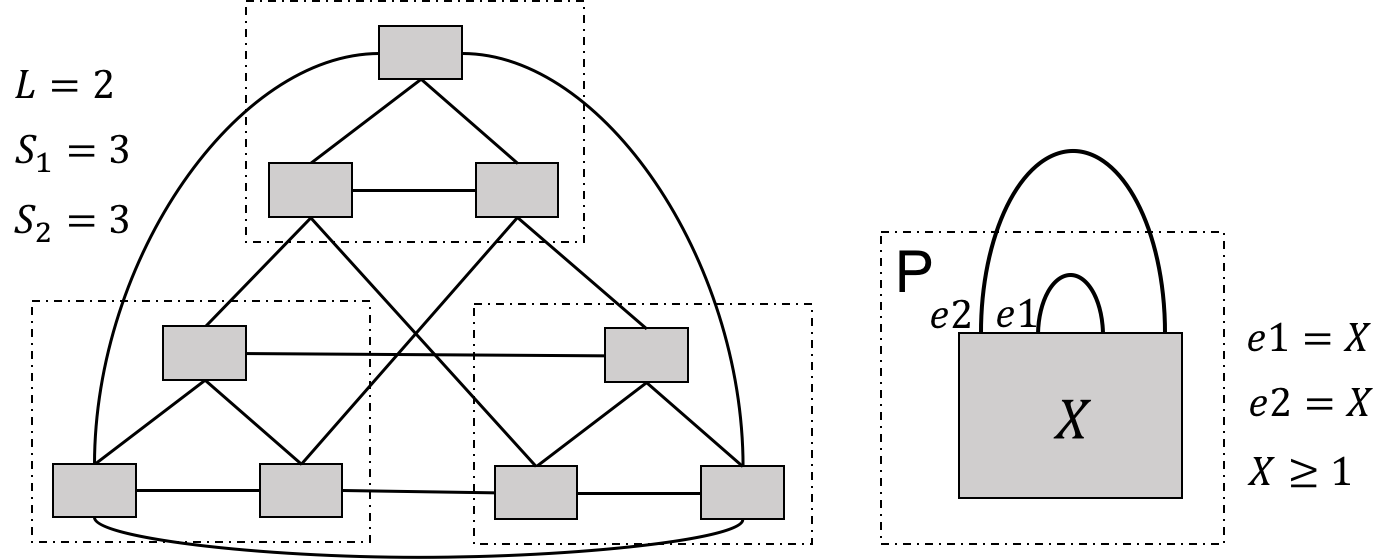
\includegraphics[width=\linewidth]{figures/hyperx}
  \end{minipage}%

  \vspace{1em}
  \begin{minipage}[t]{\linewidth}
    \hdr{BCube}{}
    \vspace{.1em}
    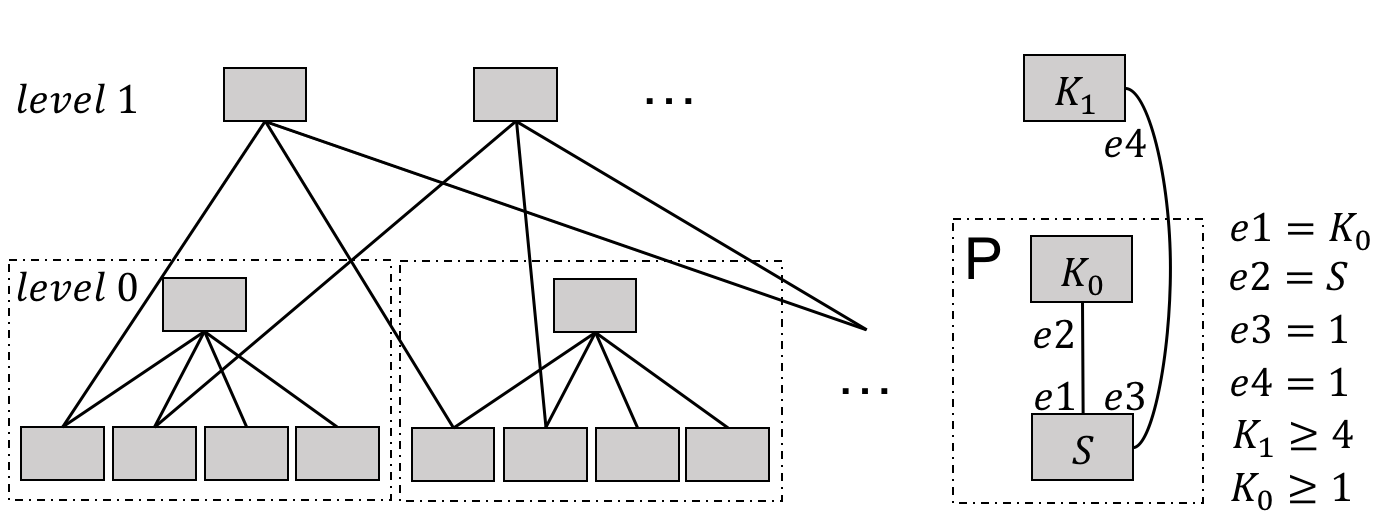
\includegraphics[width=\linewidth]{figures/bcube}
  \end{minipage}%


  \caption{Example abstractions for HyperX and BCube.}
  \label{fig:example-abstractions}
  \vspace{-.8em}%
\end{figure}

%To stress our abstractions and analysis, we consider additional topologies from the literature.

\para{Recursive Topologies}
These topologies include BCube~\cite{bcube} and DCell~\cite{dcell}. Each topology includes a recursion depth parameter ($k$), which we fixed while abstracting them. For a recursive topology with depth $k$, we model it as an abstract topology consisting of a pod to represent all depth $k-1$ subcomponents. This allows for safe expansion within a subcomponent, but does not allow changing the recursion depth dynamically.
For BCube, we model each tier of the data center as a separate role. Figure~\ref{fig:example-abstractions} shows an example of a BCube abstraction for $k=1$.

\para{Hypercube Topologies}
Hypercube variants can be used as an alternative to Clos-style topologies for networks with port density routers. The HyperX~\cite{hyperx} topology generalizes the hypercube and butterfly topologies and includes parameters $L$ for the lattice dimension of the network, and $S_i$ for the node multiplicity of each dimension $i$.
%$K_i$ for the bandwidth of links for each dimension,
%and $T$ for the number of terminal nodes (servers) connected to each router.
For a fixed number of dimensions $L$, we abstract each full mesh of $S_L$ nodes into its own abstract node. Nodes in dimension $S_{x-1}$ are abstracted using pods of abstract nodes from dimension $S_x$. Figure~\ref{fig:example-abstractions} shows an example for $L=2$.
%For all hypercube variants, the fault-tolerance analysis is precise.

\para{Results}
The bottom part of Figure~\ref{fig:analysis-precision} shows the results for all types of topologies coupled with shortest-path routing. (Valley-free routing is not meaningful for non-tree-based topologies.) For all tree-based topologies, the analysis is precise for determining reachability, but for three of them, it does not compute a tight bound for disjoint paths for all router pairs. Specifically, it underestimates ToR-to-spine paths; it fails to account for some circuitous paths that traverse another spine because it could not disambiguate two concrete spines that map to the same abstract role.
%
For instance, for the fat tree topology~\cite{fattree}, it only finds 1 path between any ToR and any Spine when there should always be at least two. However, in this case the analysis computes the correct worst case connectivity between any source ToR and any other destination aggregation or ToR router. A similar pattern occurs with other tree-based topologies.
%
%For all fat tree variants, the analysis correctly computes the number of ToR to ToR disjoint paths, but can lose precision between ToR to spine routers due to valley paths. For a valley-free routing policy, the analysis is precise for ToR to spine connectivity.
For both recursive topologies, the analysis can only accurately determine reachability.
%For the BCube topology, it is able to to determine the correct number of disjoint paths between some pairs of nodes, but not all. For all hypercube topologies, \sysname's fault-tolerance analysis is precise.


%\para{Random Network Topologies}
%
%Random networks such as Scafida and Jellyfish have seen a great deal of interest in academia. These topologies were designed with an eye towards incremental expansion and are based on probabilistic arguments of bisection bandwidth in random regular graphs. However, because the topologies are created randomly, there are no hard guarantees on the connectivity between different routers. We can trivially represent these networks using a \emph{one big router} abstraction for the entire network.


\subsection{Synthesis time}

\begin{figure}[t!]
  \subcaptionbox{Data center}
    {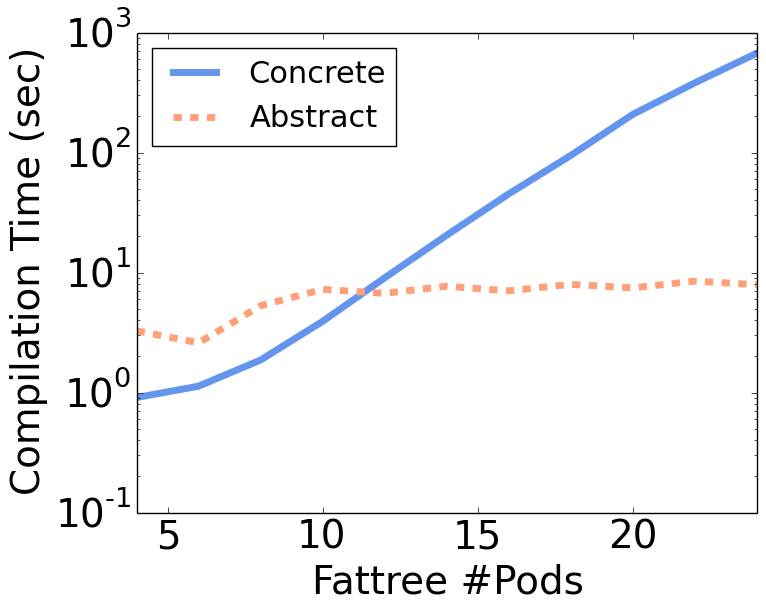
\includegraphics[width=.49\columnwidth]{figures/Fattree-time.png}}
  \subcaptionbox{Backbone}
    {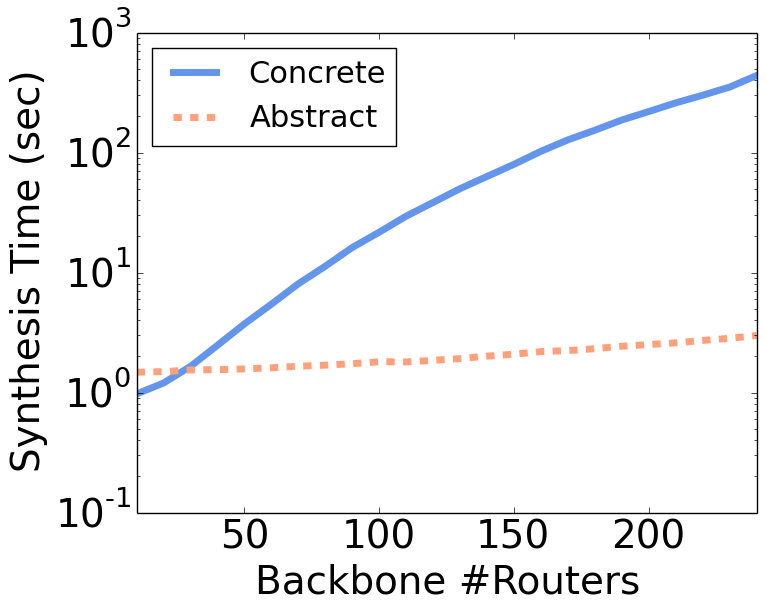
\includegraphics[width=.49\columnwidth]{figures/backbone-time.png}} \\
  \vspace{-.6em}
  \caption{Concrete vs. Abstract Synthesis Time. \label{fig:compilation-times}}
  \vspace{-1.2em}
\end{figure}

\begin{figure}[t!]
  \subcaptionbox{Data center}
    {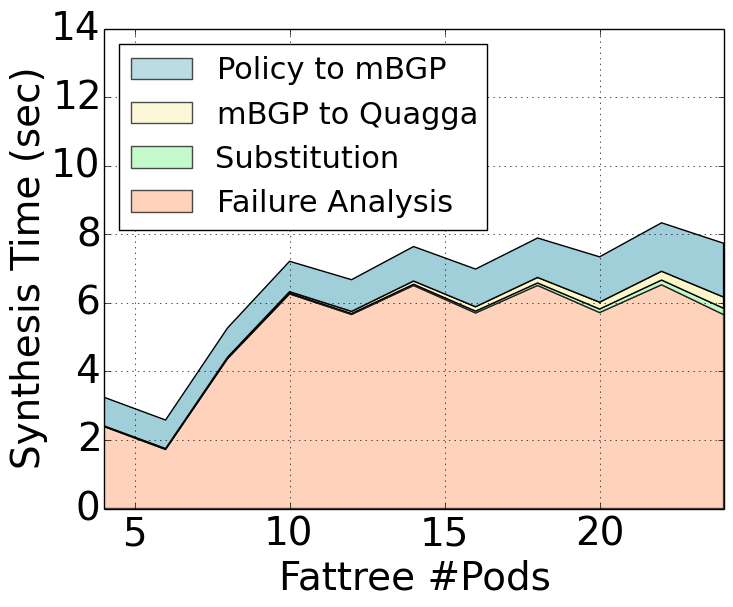
\includegraphics[width=.49\columnwidth]{figures/Fattree-analysis-time.png}}
  \subcaptionbox{Backbone}
    {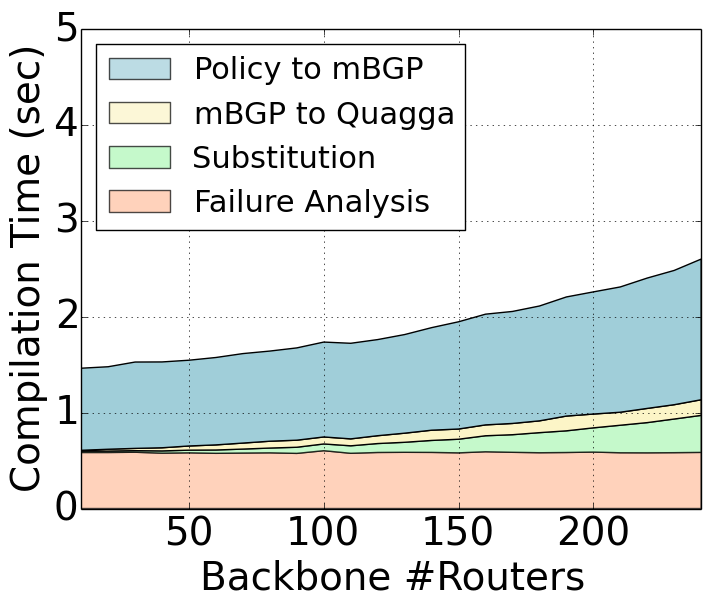
\includegraphics[width=.49\columnwidth]{figures/backbone-analysis-time.png}} \\
  \vspace{-.6em}
  \caption{Abstract Synthesis Time by Phase. \label{fig:abstract-breakdown}}
  \vspace{-.4em}
\end{figure}


We evaluate generation time in \sysname both with and without abstraction using routing policy for backbone and data center networks inspired by configurations obtained from a large cloud provider. For both types networks, we fix the routing policy and scale the size of the topology.


\para{Topologies}

Routers in the data centers run BGP using unique AS numbers and connect to multiple external neighbors. The routers aggregate some prefix blocks when announcing them to external neighbors, and keep some prefixes internal. The data center prefers that traffic leave through certain neighbors over others and should not transit traffic between neighbors. The policy also prevents routers from using external neighbors to reach ``private" destinations  (i.e., those in the IP address space reserved for private use).
%
We use a fat tree~\cite{fattree} and scale it by increasing the number of pods. The abstract topology uses one abstract node for each tier with additional nodes for local and global ToRs.

%\para{Backbone}

The backbone policy classifies neighbors into several categories based on commercial relationship~\cite{gao-rexford} and prefers paths through them in order. Like the data center, it blocks private destinations from neighbors, drops transit traffic between certain neighbors but not others, and aggregates internal prefixes at the border of the network.
%
We scale the backbone network from 10 to 240 routers. To abstract it, we split it into two parts: border routers that connect to external neighbors and an internal core. We use one abstract node for the border routers and one for the network core with mincut annotations both within the core and between the core and border roles. For neighbors, there is one abstract role per commercial category.

\para{Results}

Figure~\ref{fig:compilation-times} shows total configuration generation time for \sysname vs the concrete network synthesis tool \Propane. All experiments were run on an 8 core, 2.4 GHz Intel i7 processor machine running Mac with 16GB of Ram.

For both networks, the abstract synthesis is slightly slower than concrete synthesis for small topologies due to the overhead of the fault-tolerance analysis. However, as the topology size increases, abstract synthesis becomes orders of magnitude faster. In all cases for both networks, it takes less than 10 seconds to complete.

Figure~\ref{fig:abstract-breakdown} shows the relative time taken by each phase of \sysname. The fault-tolerance analysis takes the most time, but that does not depend on the number of concrete nodes in the network, and thus is largely a fixed cost. In particular, the number of calls to $\nu$Z remains constant across topology size. The seesaw behavior for the data center networks results from differences in time taken by $\nu$Z to minimize similar constraints with different values.

\subsection{Incrementality}
\label{sec:incrementality}

\sysname's compilation strategy guarantees that network evolution requires configuration changes only for nodes that acquire or lose a neighbor. We experimentally confirmed that our implementation provides this guarantee. For the networks we studied above, we made a range of changes, including adding and removing routers and pods and changing prefixes that routers originate. In each case, we found the guarantee to hold; for prefix changes, only the originator's configuration changed. In contrast, all router configurations were modified with \Propane because it heavily uses prefix lists which are sensitive to such changes. While \Propane may be made friendlier to network evolution (e.g., prefix lists are unnecessary at aggregation routers), its fundamental limitation will remain because it does not understand roles and the network's structure that \sysname leverages.



%=====================================================
%
%
%  **Related Work**
%
%
%=====================================================

\section{Related Work}
\label{sec:related}

%Our work is related to three threads of prior work.

\para{Network synthesis} Many recent systems focus on allowing operators to specify their policies at a high level of abstraction. These can be classified into two classes. The first class targets networks based on SDN (software-defined networking) and generates dataplane rules~\cite{foster:merlin,fattire,netgen}. The second class, to which our work belongs, targets conventional networks and generates control-plane router configurations~\cite{synet-synthesis,narain+:configassure,propane}.
%, based on which the routers interact and compute forwarding rules~\cite{propane,narain:lisa05,narain+:configassure}.
%Almost all large networks (old or new) use the conventional paradigm because that scales better~\cite{bgp-in-dc}.

While we borrow much from existing configuration synthesis work, especially \Propane~\cite{propane}, our goal is to generate role templates from abstract topologies, rather than router configurations from concrete topologies.
This goal aligns better with operators' mental models and tools and permits network evolution with minimal disruption. In the process, we develop new abstractions for network topologies, compilation algorithms that generate templates, and analysis techniques that operate over classes of networks.

\para{Topology design} Network topology design, especially for data centers, is another active research area, with researchers exploring designs with different properties~\cite{fattree,facebook-fattree,f10-fattree,vl2-fattree,bcube,dcell,hyperx,butterfly}. We do not develop new designs but develop abstractions that can capture these designs (and their evolution).

%While not the focus of this paper, \sysname can enable operators to pick the right design for their networks, more quickly and with stronger guarantees. Today, when picking a design, operators analyze its multiple concrete instantiations because available analysis tools work with concrete topologies~\cite{condor}. This process is time-consuming and not fool-proof; analyzing large, concrete topologies (with potentially thousands of nodes) takes a lot of time and the analysis does not cover the entire space of topologies that may arise.

\para{Network verification}
A complementary approach to reducing configuration errors is to analyze the forwarding rules or the configuration of a network to ensure the absence of (a class of) bugs~\cite{anteater,hsa,veriflow,feamster+:rcc,ipassure,batfish,bagpipe,arc,era,surgery,coalgebraic}. Our focus, in contrast, is on a correct-by-construction approach. It has the downside that operators must express policies in a new language, but it saves them from the challenging and time-consuming task of manual configuration generation.


%\para{Configuration synthesis}
%ConfigAssure~\cite{narain:lisa05,narain+:configassure}
%is another system designed to
%help users define and debug low-level router
%configurations.  Inputs to
%ConfigAssure include a \emph{configuration database}, which contains a
%collection of tuples over constants and configuration variables, and a
%\emph{requirement}, which is a set of constraints.
%%
%The authors use a combination of logic programming and
%SAT solving to find concrete values for configuration variables.
%ConfigAssure handles configuration for a wide range of protocols and many
%different concerns.  In contrast, the scope of \sysname is much
%narrower.  In return, \sysname offers compact, higher-level
%abstractions customized for our domain, such as regular paths, as well
%as domain-specific analyses customized to those abstractions, such as
%our failure safety analysis.  The implementation technology is also
%entirely different, as we define algorithms over automata and graphs
%as opposed to using logic programming and SAT-based model-finding.


%=====================================================
%
%
%  **Conclusions**
%
%
%=====================================================

\section{Conclusions}
\label{sec:conclusions}

To help configure large networks correctly, we develop \sysname, the first system that can generate role templates from high-level specifications of network topology and policy. \sysname is based on new abstractions for capturing network topologies, and their evolution, and algorithms to analyze the combined impact of topology and routing policy on the network's fault tolerance. Our analysis operates entirely in the abstract domain and guarantees correctness for all concrete instantiations of the topology. Experiments with many types of real-world topologies and policies show that our abstractions and analysis are effective and that, for large networks, configuration synthesis is two orders of magnitude faster than systems that operate over concrete topologies.

\para{Acknowledgments}
We thank the many network engineers, especially George Chen and Lihua Yuan, who pointed out the importance of working with abstract topologies. 
We also thank the PLDI reviewers, and especially our shepherd Alexandra Silva for comments on the paper. This work is supported in part by the National Science Foundation award CNS-1161595 and Cisco award 677002.


%=====================================================
%
%
%  **Bibliography**
%
%
%=====================================================

\balance


\bibliographystyle{abbrvnat}
\bibliography{references}


%=====================================================
%
%
%  **Appendix**
%
%
%=====================================================


\end{document}
